%-----------------------------------------------------------------------------%
\chapter{\babTiga}
\label{bab:3}
%-----------------------------------------------------------------------------%
Bab ini menjelaskan mengenai desain dari sistem yang dibuat untuk menjalankan dan
menyelesaikan penelitian. Berikut ini diagram alur yang memvisualisasikan gambaran besar
tahapan-tahapan yang dilakukan. Penjelasan setiap tahap disajikan pada paparan subbab selanjutnya.

%-----------------------------------------------------------------------------%
%-----------------------------------------------------------------------------%
\section{Desain Penelitian}
\label{sec:desainPenelitian}
%-----------------------------------------------------------------------------%
Penelitian dimulai dengan mendefinisikan latar belakang permasalahan penelitian. Hal tersebut bertujuan untuk menentukan fokus permasalahan yang akan dicoba dijawab dalam penelitian. Permasalahan akan didefinisikan dalam bentuk pertanyaan dan batasan penelitian. Berikutnya, tujuan penelitian ditentukan serta langkah dan metodologi penyelesaian permasalahannya.

%-----------------------------------------------------------------------------%
\section{Tinjauan Pustaka}
\label{sec:tinjauanPustaka}
% Hal baru di template 2017
%-----------------------------------------------------------------------------%
Studi literatur terkait materi-materi yang relevan dengan penelitian dilakukan untuk menunjang penelitian. Topik-topik relevan yang dipelajari ialah \textit{Moodle}, \textit{Machine Learning}, Deteksi non-compliance, \textit{Log Processing}, dan \textit{eLearning}. Hasil dari studi literatur ini sebagai landasan dalam pengembangan model.

%-----------------------------------------------------------------------------%
\section{Sumber Data Log}
\label{sec:sumberDataLog}
%-----------------------------------------------------------------------------%
Bagian ini menguraikan secara mendalam mengenai dua jenis data utama yang digunakan dalam penelitian: data log aktivitas sistem \textit{Moodle} dan data artifisial. 

\textbf{Data Log Moodle:} \\
Data log \textit{Moodle} diambil langsung dari sistem yang dikelola oleh tim ITF Fasilkom UI dan disimpan di Lumbung Storage Cloud. Data tersebut telah melalui proses anonimisasi dengan menggantikan identitas asli pengguna (seperti \textit{username} dan nama lengkap) dengan \textit{user\_id}, guna menjaga privasi pengguna.

\textbf{Data Artifisial:} \\
Sementara itu, data artifisial dikembangkan untuk keperluan pengembangan model deteksi \textit{non-compliance}. Dalam penelitian ini, model dikembangkan sepenuhnya menggunakan data artifisial sehingga memungkinkan eksplorasi berbagai skenario ekstrem. Pada tahap akhir, model akan dievaluasi dengan data log riil untuk menguji kemampuannya dalam mendeteksi kasus kecurangan yang terjadi di dunia nyata.

\subsection{Data Log Moodle Riil: Deskripsi (periode, jumlah event/user, fitur utama), Proses Akuisisi, Kebijakan Anonimisasi \& Etika.}
\label{sec:logRiil}
Subbab ini menjelaskan mengenai data log yang diambil langsung dari sistem \textit{Moodle}, yang dikelola oleh tim ITF Fasilkom UI dan disimpan pada Lumbung Storage Cloud (mirip dengan platform penyimpanan seperti Google Drive). Data yang digunakan telah melalui proses anonimisasi, di mana identitas asli pengguna (username atau nama lengkap) tidak disertakan, melainkan hanya diwakili oleh \textit{user\_id}.

%-----------------------------------------------------------------------------%
\subsubsection{Deskripsi Data}
\label{sec:deskripsiData}
Data log \textit{Moodle} terdiri dari beberapa tabel utama yang masing-masing menyimpan informasi berbeda terkait aktivitas pengguna dan kuis. Berikut adalah rincian kolom-kolom yang terdapat dalam tiap tabel:

\textbf{mdl\_question\_usages} \\
Kolom: \textit{question\_usage\_id}, \textit{context\_id} \\
Menyimpan informasi terkait konteks penggunaan pertanyaan dalam kuis.

\textbf{mdl\_quiz\_grades} \\
Kolom: \textit{quiz\_grades\_id}, \textit{quiz\_id}, \textit{user\_id}, \textit{final\_grade} \\
Berisi nilai akhir dari masing-masing kuis yang diambil oleh pengguna.

\textbf{mdl\_question\_attempt\_steps} \\
Kolom: \textit{question\_step\_id}, \textit{question\_attempt\_id}, \textit{sequencenumber}, \textit{state}, \textit{timecreated} \\
Mencatat tiap langkah (\textit{step}) dalam upaya pengerjaan soal, termasuk status dan waktu pembuatan.

\textbf{mdl\_quiz\_attempts} \\
Kolom: \textit{attempt\_id}, \textit{quiz\_id}, \textit{user\_id}, \textit{question\_usage\_id}, \textit{timestart}, \textit{timefinish}, \textit{state}, \textit{sumgrades} \\
Menggambarkan detail setiap upaya pengerjaan kuis, termasuk waktu mulai, waktu selesai, status, dan jumlah nilai yang diperoleh. \\
Catatan: Terdapat anomali pada \textit{timefinish} (misalnya timestamp 1970-01-01) yang kemungkinan menunjukkan upaya kuis yang belum selesai atau default nilai dari Unix epoch.

\textbf{mdl\_question\_answers} \\
Kolom: \textit{question\_answers\_id}, \textit{questionid}, \textit{answer\_text}, \textit{fraction} \\
Menyimpan data mengenai jawaban yang diberikan pada tiap pertanyaan, termasuk teks jawaban dan bobot nilai yang terkait.

\textbf{mdl\_question\_attempt\_step\_data} \\
Kolom: \textit{step\_data\_id}, \textit{question\_step\_id}, \textit{name}, \textit{value} \\
Menyimpan data tambahan terkait langkah pengerjaan soal, yang dapat berupa nilai-nilai pendukung dari proses evaluasi.

\textbf{mdl\_quiz} \\
Kolom: \textit{quiz\_id}, \textit{course}, \textit{quiz\_name}, \textit{timeopen}, \textit{timeclose}, \textit{timelimit} \\
Berisi informasi dasar mengenai kuis, termasuk mata kuliah, nama kuis, serta waktu buka dan tutup kuis.

\textbf{mdl\_sessions} \\
Kolom: \textit{session\_id}, \textit{user\_id}, \textit{timecreated}, \textit{lastip}, \textit{sessdata} \\
Mencatat aktivitas sesi pengguna, mulai dari waktu pembuatan sesi hingga informasi terkait IP dan data sesi lainnya.

%-----------------------------------------------------------------------------%
\subsubsection{Rentang Waktu dan Skala Dataset}
\label{sec:rentangWaktuSkalaDataset}
Data log \textit{Moodle} mencakup periode hampir 10 tahun, dengan rentang data keseluruhan dari tanggal 31 Juli 2015 hingga 22 Februari 2025. Secara spesifik:

\textbf{mdl\_question\_attempt\_steps:} \\
Rentang waktu: 29 Agustus 2015 – 22 Februari 2025 \\
Durasi: sekitar 3.565 hari

\textbf{mdl\_quiz\_attempts:} \\
Rentang waktu untuk \textit{timestart}: 31 Juli 2015 – 22 Februari 2025 \\
Rentang waktu untuk \textit{timefinish}: (dengan catatan anomali timestamp 1970 sebagai default) hingga 22 Februari 2025 \\
Durasi: sekitar 3.594 hari (mengabaikan nilai default 1970)

\textbf{mdl\_sessions:} \\
Rentang waktu: 17 Maret 2020 – 22 Februari 2025 \\
Durasi: sekitar 1.803 hari

Skala data secara keseluruhan meliputi:
\begin{itemize}
    \item Total kuis yang diambil: 446.720 upaya
    \item Jumlah pengguna unik: 5.562
    \item Jumlah kuis unik: 6.304
    \item Jumlah langkah pertanyaan: 22.192.809
\end{itemize}

%-----------------------------------------------------------------------------%
\subsubsection{Cakupan Mata Kuliah dan Pola Penggunaan}
\label{sec:cakupanMataKuliahPolaPenggunaan}
Data ini mencakup aktivitas di lebih dari 140 Mata Kuliah unik, dengan variasi ukuran kelas:

\textbf{Ukuran Mata Kuliah:}
\begin{itemize}
    \item Mata Kuliah besar (300+ mahasiswa): sekitar 10 Mata Kuliah
    \item Mata Kuliah menengah (100-300 mahasiswa): sekitar 30 Mata Kuliah
    \item Mata Kuliah kecil (<100 mahasiswa): sekitar 100 Mata Kuliah
    \item Mata Kuliah sangat kecil (<10 mahasiswa): sekitar 15 Mata Kuliah
\end{itemize}

\textbf{Contoh Mata Kuliah dengan aktivitas tinggi:}
\begin{itemize}
    \item Mata Kuliah 3836: 453 peserta, 5.544 upaya (rata-rata 12,24 upaya per pengguna)
    \item Mata Kuliah 3634: 442 peserta, 5.902 upaya (rata-rata 13,35 upaya per pengguna)
    \item Mata Kuliah 3723: 390 peserta, 3.829 upaya (rata-rata 9,56 upaya per pengguna)
    \item Mata Kuliah 3640: 386 peserta, 4.463 upaya (rata-rata 11,56 upaya per pengguna)
    \item Mata Kuliah 3636: 382 peserta, 761 upaya (rata-rata 1,99 upaya per pengguna)
\end{itemize}

Pola penggunaan kuis menunjukkan perbedaan yang signifikan antar Mata Kuliah. Beberapa Mata Kuliah hanya mencatat satu upaya per pengguna, sedangkan Mata Kuliah lain mencatat rata-rata 10 upaya atau lebih, yang mengindikasikan adanya kuis latihan atau kebijakan pengulangan untuk meningkatkan pemahaman materi.

%-----------------------------------------------------------------------------%
\subsubsection{Proses Akuisisi dan Kebijakan Anonimisasi}
\label{sec:prosesAkuisisiKebijakanAnonimisasi}
Data log \textit{Moodle} diakuisisi secara langsung dari sistem \textit{Moodle} oleh tim ITF Fasilkom UI dan kemudian disimpan di Lumbung Storage Cloud. Proses akuisisi melibatkan:

\textbf{Pengambilan Data:} \\
Data diekstraksi dari server \textit{Moodle} dengan menggunakan prosedur logging yang telah ditetapkan, memastikan setiap aktivitas terekam secara lengkap.

\textbf{Pengiriman dan Penyimpanan:} \\
Data dikirim dan disimpan secara terpusat di Lumbung Storage Cloud yang merupakan repository internal Fasilkom UI, menjamin keamanan dan integritas data.

\textbf{Anonimisasi:} \\
Untuk melindungi privasi pengguna, data telah diproses sehingga informasi identitas pribadi (username, nama lengkap, dan data sensitif lainnya) dihilangkan. Hanya \textit{user\_id} yang tetap dipertahankan untuk keperluan analisis. Hal ini sesuai dengan standar etika penelitian dan kebijakan perlindungan data yang berlaku.

\textbf{Pertimbangan Etika:} \\
Penggunaan data riil ini telah mempertimbangkan aspek etika dan regulasi perlindungan data. Kebijakan anonimisasi yang diterapkan memastikan bahwa data tidak dapat dikaitkan langsung dengan individu tertentu, sehingga menjaga kerahasiaan dan privasi pengguna.

%-----------------------------------------------------------------------------%
\subsection{Data Artifisial: Peran dan Tujuan Penggunaannya}
\label{sec:dataArtifisial}
%-----------------------------------------------------------------------------%
Subbab ini memaparkan peran dan tujuan penggunaan data artifisial dalam penelitian. Data artifisial dirancang untuk menggantikan penggunaan data riil pada tahap pengembangan model, dengan alasan-alasan sebagai berikut:

\begin{enumerate}
    \item \textbf{Kontrol Variabel dan Simulasi Skenario Ekstrem:} \\
    Data artifisial memungkinkan penciptaan skenario perilaku pengguna yang ekstrem atau tidak biasa, yang mungkin jarang terjadi pada data log riil. Dengan demikian, model dapat dilatih untuk mengenali pola-pola \textit{non-compliance} secara lebih spesifik dan mendalam.
    
    \item \textbf{Pengembangan Model yang Terarah:} \\
    Dalam penelitian ini, pengembangan model dilakukan sepenuhnya dengan menggunakan data artifisial. Pendekatan ini memberikan fleksibilitas dalam mengatur parameter dan iterasi pelatihan, serta mengurangi risiko \textit{overfitting} pada data riil yang belum terlabel dengan jelas.
    
    \item \textbf{Evaluasi Model dengan Data Riil:} \\
    Setelah model dioptimasi dengan data artifisial, evaluasi akhir akan dilakukan dengan menerapkan model pada data log asli. Langkah ini bertujuan untuk mengukur sejauh mana model dapat mendeteksi kasus kecurangan yang benar-benar terjadi di lingkungan sistem \textit{Moodle}, sehingga memberikan validasi nyata terhadap efektivitas pendekatan yang digunakan.
    
    \item \textbf{Pendekatan Metodologis dalam Pembuatan Data Artifisial:} \\
    Data artifisial dihasilkan melalui kombinasi simulasi berbasis aturan dan proses stokastik, yang disesuaikan dengan pola penggunaan yang ditemukan dalam data log riil. Pendekatan ini memastikan bahwa data artifisial tidak hanya mereplikasi kondisi normal, tetapi juga memasukkan skenario \textit{non-compliance} yang relevan untuk pengembangan model.
\end{enumerate}

Dengan demikian, penggunaan data artifisial dalam penelitian ini memberikan keuntungan dalam hal kontrol variabilitas dan eksplorasi skenario ekstrem, serta mempercepat proses pengembangan model. Evaluasi akhir dengan data log riil akan menjadi tolok ukur untuk menilai kemampuan model dalam mendeteksi kecurangan yang terjadi secara nyata dalam sistem \textit{Moodle}.

%-----------------------------------------------------------------------------%
\section{Pra-pemrosesan Data Log}
\label{sec:praPemrosesanDataLog}
%-----------------------------------------------------------------------------%
Tahap pra-pemrosesan data log merupakan fondasi penting dalam penelitian ini, di mana seluruh data mentah—baik yang dihasilkan oleh sistem \textit{Moodle} maupun data artifisial—diolah agar memiliki kualitas, konsistensi, dan keseragaman yang diperlukan untuk analisis selanjutnya. Proses ini tidak hanya bertujuan untuk mengurangi noise dan inkonsistensi, tetapi juga untuk memastikan bahwa fitur-fitur yang dihasilkan mencerminkan karakteristik perilaku pengguna secara akurat. Implementasi proses ini dilakukan melalui beberapa modul skrip, antara lain \texttt{preprocess\_features.py}, \texttt{feature\_eng.py}, dan \texttt{fixed\_extraction.py}. Langkah-langkah berikut diambil dengan dasar metodologis yang defendable secara ilmiah:

%-----------------------------------------------------------------------------%
\subsection{Pembersihan Data (Data Cleaning)}
\label{sec:pembersihanData}
%-----------------------------------------------------------------------------%
\textbf{Penanganan Missing Values:} \\
Data log sering kali mengandung nilai yang hilang (\textit{missing values}) karena ketidakteraturan dalam pencatatan event atau error saat pengambilan data. Dalam pipeline, nilai yang tidak terisi diimputasi dengan metode penggantian menggunakan nilai default (misalnya, 0) atau perhitungan statistik (rata-rata/median) ketika relevan. Misalnya, dalam skrip \texttt{preprocess\_features.py}, setelah ekstraksi fitur, seluruh nilai NaN diisi dengan nol untuk memastikan tidak ada celah data yang dapat mengganggu analisis model.

\textbf{Filtering Data yang Tidak Relevan:} \\
Dalam konteks deteksi kecurangan, tidak seluruh event log memiliki nilai informasi yang sama. Oleh karena itu, dilakukan penyaringan untuk:
\begin{itemize}
    \item Mengabaikan event dengan atribut tertentu (misalnya, field \textit{contextlevel} yang bernilai 'system') karena event ini tidak mewakili aktivitas pengguna pada kuis.
    \item Menghapus entri dengan \textit{user\_id} yang null, mengingat identifikasi pengguna merupakan variabel kunci dalam analisis pola perilaku.
\end{itemize}

%-----------------------------------------------------------------------------%
\subsection{Transformasi dan Normalisasi Data}
\label{sec:transformasiNormalisasiData}
%-----------------------------------------------------------------------------%
\textbf{Unifikasi Format Waktu dan Normalisasi Zona Waktu:} \\
Data log mengandung timestamp yang berasal dari sumber atau zona waktu yang berbeda. Untuk memastikan keseragaman, seluruh timestamp dikonversi ke dalam format numerik, seperti Unix timestamp (atau ISO 8601 jika diperlukan), melalui fungsi konversi di \texttt{preprocess\_features.py}. Proses ini juga melibatkan normalisasi zona waktu agar seluruh event log dapat dibandingkan secara akurat dalam kerangka waktu yang sama.

\textbf{Parsing Nested Fields:} \\
Banyak kolom dalam data log disimpan dalam bentuk string yang merepresentasikan array atau dictionary (misalnya, sequence navigasi atau transition times). Menggunakan fungsi seperti \texttt{ast.literal\_eval}, skrip melakukan parsing terhadap string tersebut sehingga struktur data yang tersusun (list atau dictionary) dapat diekstraksi. Proses ini memungkinkan perhitungan fitur statistik seperti panjang sequence, entropi, dan jumlah revisits, yang esensial untuk mendeteksi pola aktivitas pengguna.

%-----------------------------------------------------------------------------%
\subsection{Ekstraksi Fitur dan Deteksi Outlier}
\label{sec:ekstraksiFiturDeteksiOutlier}
%-----------------------------------------------------------------------------%
Setelah data dibersihkan dan ditransformasikan, tahap selanjutnya adalah ekstraksi fitur, di mana fitur-fitur dasar dan lanjutan dihasilkan untuk mendukung proses pelatihan model deteksi kecurangan. Dalam pipeline, ekstraksi fitur dilakukan melalui modul \texttt{feature\_eng.py} dan \texttt{fixed\_extraction.py}, dengan beberapa langkah sebagai berikut:

\textbf{Fitur Dasar:} \\
Fitur seperti jumlah percobaan kuis, rata-rata waktu pengerjaan, total waktu, serta statistik minimum dan maksimum dihitung dari data log kuis. Contoh implementasi terdapat pada fungsi \texttt{extract\_basic\_statistics()} di \texttt{feature\_eng.py}, yang juga menyertakan agregasi data per pasangan user-kuis.

\textbf{Fitur Sequence:} \\
Dari data navigasi dan jawaban, diekstraksi fitur-fitur seperti:
\begin{itemize}
    \item Panjang sequence dan jumlah pertanyaan unik: Mengukur seberapa panjang dan bervariasinya aktivitas navigasi pengguna.
    \item Linearity: Menghitung seberapa berurutan langkah-langkah yang diambil, menggunakan perhitungan rasio antara pertanyaan unik dan total langkah.
    \item Revisits: Penghitungan jumlah revisits atau langkah yang diulang, sebagai indikasi pola abnormal.
\end{itemize}
Fungsi \texttt{extract\_navigation\_features()} dalam \texttt{fixed\_extraction.py} mengilustrasikan bagaimana fitur-fitur tersebut dihitung dengan memanfaatkan evaluasi list dari sequence.

\textbf{Deteksi Outlier pada Fitur Waktu:} \\
Pada ekstraksi fitur waktu, dilakukan perhitungan statistik seperti rata-rata, standar deviasi, nilai minimum dan maksimum dari durasi pengerjaan soal. Selain itu, skrip juga menghitung jumlah event dengan durasi sangat pendek (misalnya, < 5 detik) dan sangat panjang (misalnya, > 600 detik).

Berikut adalah cuplikan kode dari fungsi \texttt{extract\_timing\_features()} yang digunakan untuk mendeteksi pola waktu yang abnormal, yang dapat dijadikan indikator outlier:

\begin{verbatim}
def extract_timing_features(time_seq):
    """Extract features from timing sequence."""
    features = {}
    
    try:
        if isinstance(time_seq, str):
            time_seq = eval(time_seq)
        time_seq = np.array(time_seq, dtype=float)
        
        features['mean_time'] = float(np.mean(time_seq))
        features['std_time'] = float(np.std(time_seq))
        features['min_time'] = float(np.min(time_seq))
        features['max_time'] = float(np.max(time_seq))
        
        # Suspicious timing patterns sebagai indikator outlier
        features['quick_answers'] = int(sum(1 for t in time_seq if t < 5))
        features['very_long_answers'] = int(sum(1 for t in time_seq if t > 600))
    except Exception as e:
        print(f"Warning: Error processing timing features: {e}")
        features['mean_time'] = 0.0
        features['std_time'] = 0.0
        features['min_time'] = 0.0
        features['max_time'] = 0.0
        features['quick_answers'] = 0
        features['very_long_answers'] = 0
    
    return features
\end{verbatim}

Nilai \texttt{quick\_answers} dan \texttt{very\_long\_answers} ini memberikan gambaran tentang berapa kali pengguna menyelesaikan bagian tertentu dengan durasi yang sangat tidak wajar, yang kemudian dapat diintegrasikan sebagai fitur untuk mendeteksi perilaku kecurangan.

\textbf{Penghitungan Similarity Features:} \\
Untuk mendeteksi kolaborasi kecurangan, pipeline menghitung matriks kemiripan (\textit{similarity matrix}) berdasarkan pola navigasi, waktu, dan jawaban antar pengguna. Fungsi \texttt{calculate\_similarity\_matrices()} di \texttt{feature\_eng.py} menghitung kemiripan menggunakan metode seperti Levenshtein distance untuk sequence navigasi dan korelasi untuk sequence waktu, kemudian hasilnya digunakan untuk menambahkan fitur agregat seperti rata-rata dan maksimum similarity antar pengguna.



%-----------------------------------------------------------------------------%

%-----------------------------------------------------------------------------%
\subsection{Checklist Pra-pemrosesan}
\label{sec:checklistPraPemrosesan}
%-----------------------------------------------------------------------------%
Untuk memastikan bahwa seluruh proses pra-pemrosesan dapat diulangi dan diverifikasi, disusunlah checklist sebagai berikut:
\begin{itemize}
    \item Konversi seluruh timestamp ke format standar (Unix timestamp atau ISO 8601).
    \item Penghapusan event dengan atribut \textit{contextlevel} bernilai 'system'.
    \item Penyaringan entri dengan \textit{user\_id} null.
    \item Parsing kolom yang berisi string representasi array/dict untuk ekstraksi fitur.
    \item Normalisasi zona waktu untuk keseragaman data.
    \item Perhitungan statistik fitur dasar dan sequence (termasuk deteksi pola outlier pada waktu).
\end{itemize}

%-----------------------------------------------------------------------------%
\subsection{Justifikasi Ilmiah}
\label{sec:justifikasiIlmiah}
%-----------------------------------------------------------------------------%
Pendekatan pra-pemrosesan yang diterapkan dalam penelitian ini didasarkan pada prinsip-prinsip \textit{data cleaning} dan \textit{feature engineering} yang telah terbukti secara empiris meningkatkan kualitas dataset dan kinerja model \textit{machine learning}.

\textbf{Pembersihan dan Transformasi:} \\
Dengan memastikan bahwa data dalam format yang konsisten dan bebas dari \textit{missing values}, variabilitas yang tidak relevan dapat diminimalkan, sehingga model tidak terdistorsi oleh noise data.

\textbf{Ekstraksi Fitur:} \\
Fitur-fitur yang diekstraksi, seperti linearity dan revisits pada sequence, memberikan representasi numerik yang dapat menggambarkan perilaku pengguna secara mendalam.

\textbf{Deteksi Outlier:} \\
Dengan mengidentifikasi event dengan durasi yang sangat singkat atau sangat panjang, pipeline mampu memberikan sinyal peringatan terhadap kemungkinan aktivitas yang tidak wajar, yang secara langsung berkontribusi pada identifikasi kecurangan.

\textbf{Reproducibility:} \\
Checklist dan struktur modular pada skrip memastikan bahwa seluruh proses dapat direplikasi dan diaudit, sehingga mendukung validitas dan reproducibility dari penelitian.

Melalui serangkaian proses yang sistematis dan berbasis algoritma yang telah teruji, tahap pra-pemrosesan ini memberikan dasar yang kuat untuk langkah-langkah selanjutnya dalam pipeline, yaitu ekstraksi fitur lanjutan, pelatihan model, dan akhirnya evaluasi deteksi kecurangan.

%-----------------------------------------------------------------------------%
\section{Perancangan dan Generasi Data Log Moodle Artifisial}
\label{sec:perancanganGenerasiDataArtifisial}
%-----------------------------------------------------------------------------%
Subbab ini menjelaskan secara mendalam mengenai rancangan, implementasi, dan validasi data log \textit{Moodle} artifisial yang digunakan untuk mengembangkan model deteksi \textit{non-compliance}. Pendekatan yang diterapkan dikenal dengan istilah \textit{Skenario Perilaku Sintetik}, yaitu simulasi aktivitas pengguna (baik perilaku normal maupun \textit{non-compliance}) melalui algoritma yang menggabungkan simulasi berbasis aturan dan proses stokastik. Data artifisial ini tidak hanya mereplikasi aktivitas log riil, tetapi juga memungkinkan eksplorasi skenario ekstrem yang jarang terekam pada data nyata, seperti koordinasi kelompok kecurangan dengan pola sinkronisasi tinggi.

%-----------------------------------------------------------------------------%
\subsection{Definisi Operasional Skenario Perilaku Sintetik}
\label{sec:definisiOperasionalSkenarioPerilakuSintetik}
%-----------------------------------------------------------------------------%
Skenario Perilaku Sintetik didefinisikan sebagai rangkaian aturan dan mekanisme yang dirancang untuk mereplikasi pola aktivitas pengguna pada sistem \textit{Moodle}, baik dalam kondisi normal maupun \textit{non-compliance} (kecurangan). Pendekatan ini mengintegrasikan simulasi berbasis aturan dengan proses stokastik, sehingga memungkinkan pembentukan data log artifisial yang tidak hanya mereplikasi aktivitas log riil, tetapi juga dapat mengeksplorasi skenario ekstrem yang jarang terekam dalam data nyata.

\textbf{Perilaku Normal:} \\
Pada skenario perilaku normal, aktivitas pengguna dirancang untuk mencerminkan dinamika berpikir yang alami, yang ditandai dengan:
\begin{itemize}
    \item Variasi Urutan Navigasi: Pengguna normal menunjukkan urutan akses pertanyaan yang bervariasi, dengan kemungkinan revisi jawaban yang berbeda-beda antar sesi. Hal ini menggambarkan proses evaluasi internal yang dinamis.
    \item Variasi Pola Jawaban: Pola jawaban mencerminkan respon acak yang wajar, dengan proporsi jawaban benar dan salah yang bervariasi secara natural.
    \item Waktu Pengerjaan yang Variatif: Interval waktu antar pertanyaan bervariasi, mencerminkan kecepatan berpikir dan penyesuaian terhadap tingkat kesulitan pertanyaan. Distribusi waktu pengerjaan ini umumnya menunjukkan standar deviasi yang wajar.
\end{itemize}

\textbf{Perilaku Non-Compliance (Kecurangan):} \\
Pada skenario \textit{non-compliance}, pola aktivitas sengaja diatur untuk menciptakan indikasi kecurangan, dengan karakteristik sebagai berikut:
\begin{itemize}
    \item Kesamaan Navigasi: Urutan pertanyaan yang diakses oleh pengguna dalam kelompok kecurangan sangat mirip, termasuk adanya revisi yang identik antar anggota kelompok.
    \item Konsistensi Jawaban: Pola jawaban menunjukkan tingkat keseragaman yang tinggi. Misalnya, terdapat kecenderungan anggota kelompok secara bersama-sama memberikan jawaban salah pada pertanyaan-pertanyaan sulit.
    \item Sinkronisasi Waktu yang Tidak Wajar: Interval waktu antar pertanyaan hampir seragam antar pengguna. Dalam beberapa kasus, terdapat kelompok yang menyelesaikan kuis secara bersamaan dalam waktu kurang dari 15 detik, dengan standar deviasi yang rendah, mengindikasikan adanya pola sinkronisasi yang sulit terjadi secara natural.
    \item Mekanisme Leader-Follower: Terdapat pola di mana satu anggota (leader) menyelesaikan kuis terlebih dahulu, sedangkan anggota lainnya (follower) mengikuti dengan delay yang konsisten. Pola ini menciptakan korelasi tinggi dalam waktu pengerjaan antar anggota, yang menjadi indikator kuat adanya koordinasi.
\end{itemize}

Definisi operasional ini menjadi dasar untuk memformulasikan parameter simulasi. Parameter-parameter tersebut, seperti tingkat kemiripan navigasi, delay waktu, dan distribusi jawaban, kemudian diintegrasikan dalam algoritma generasi data log artifisial. Setiap skenario diberikan label \textit{ground truth}, yang memungkinkan validasi dan evaluasi model deteksi kecurangan secara kuantitatif dan kualitatif.

%-----------------------------------------------------------------------------%
\subsection{Desain Ground Truth Artifisial}
\label{sec:desainGroundTruthArtifisial}
%-----------------------------------------------------------------------------%
Dalam proses generasi data log artifisial, setiap entitas—baik pada level sesi, upaya pengerjaan, maupun langkah pertanyaan—diberi label \textit{ground truth} yang mendefinisikan status sebagai aktivitas normal atau \textit{non-compliance}. Desain \textit{ground truth} ini tidak hanya merupakan hasil dari parameter simulasi, tetapi juga dilengkapi dengan dokumentasi yang komprehensif melalui file \texttt{cheating\_ground\_truth.md}. File ini berfungsi sebagai acuan empiris untuk validasi dan evaluasi model deteksi kecurangan.

\textbf{Komponen Utama Ground Truth:}
\begin{itemize}
    \item \textbf{Label Kecurangan:} \\
    Setiap entitas data dilengkapi dengan label:
    \begin{itemize}
        \item 0: Menunjukkan aktivitas normal.
        \item 1: Menunjukkan aktivitas \textit{non-compliance} (kecurangan), yang dihasilkan dari simulasi kelompok dengan pola sinkronisasi tinggi dan koordinasi yang jelas.
    \end{itemize}
    \item \textbf{Komposisi Dataset:} \\
    Data artifisial dihasilkan dengan proporsi tertentu antara perilaku normal dan \textit{non-compliance}. Proporsi ini dikonfigurasi dalam parameter simulasi, misalnya 10–20\% pengguna disimulasikan sebagai \textit{non-compliance}, untuk memastikan keseimbangan yang memadai dalam pelatihan dan evaluasi model.
    \item \textbf{Pencatatan Parameter Simulasi dan Contoh Kasus:} \\
    Parameter-parameter yang mendasari penetapan label \textit{ground truth} direkam secara detail, mencakup:
    \begin{itemize}
        \item Navigation Similarity: Persentase kesamaan urutan navigasi antar anggota kelompok (contoh: 96\%).
        \item Answer Pattern Similarity: Persentase kesamaan pola jawaban (contoh: 94\%).
        \item Timing Correlation: Koefisien korelasi waktu antar pertanyaan (contoh: 0.95).
        \item Standard Deviation (Avg): Rata-rata standar deviasi waktu pengerjaan per pertanyaan (contoh: 12 detik).
        \item Wrong Answer Bias: Probabilitas kesalahan terkoordinasi (contoh: 87\%).
    \end{itemize}
\end{itemize}

Nilai-nilai di atas disajikan sebagai contoh dalam file \texttt{cheating\_ground\_truth.md}. Penting untuk dicatat bahwa angka-angka tersebut merupakan representasi sample yang dapat dikonfigurasi ulang sesuai kebutuhan eksperimen, dan bukan merupakan nilai final yang harus diterapkan secara universal.

\textbf{Dokumentasi Melalui File Cheating Ground Truth:} \\
File \texttt{cheating\_ground\_truth.md} menyajikan tabel ringkasan statistik kelompok kecurangan beserta parameter-parameter yang telah diukur secara simulatif. Contoh tabel tersebut mencakup:
\begin{itemize}
    \item Kelompok Kecurangan dengan Severity Tinggi: Menunjukkan kesamaan navigasi, pola jawaban, dan korelasi waktu yang sangat tinggi, serta standar deviasi dan wrong answer bias yang rendah.
    \item Kelompok Kecurangan dengan Severity Sedang: Menunjukkan nilai yang lebih moderat, dengan delay waktu dan variansi yang lebih besar.
\end{itemize}

Dokumentasi ini menyediakan bukti empiris dan justifikasi statistik bahwa skenario \textit{non-compliance} yang disimulasikan memiliki karakteristik yang berbeda secara signifikan dari aktivitas normal. Informasi ini sangat penting untuk validasi model, karena memungkinkan perbandingan langsung antara prediksi model dengan \textit{ground truth}.

\textbf{Integrasi dan Reproducibility:} \\
\textit{Ground truth} artifisial yang terdokumentasi secara rinci ini diintegrasikan langsung ke dalam dataset log artifisial. Pendekatan ini memastikan bahwa evaluasi model dapat dilakukan secara objektif menggunakan metrik seperti precision, recall, F1-score, dan akurasi. Selain itu, pencatatan parameter simulasi dan contoh kasus dalam file \texttt{cheating\_ground\_truth.md} mendukung \textit{reproducibility} penelitian, karena eksperimen dapat diulang dengan menggunakan seed dan konfigurasi yang sama.

Dengan demikian, desain \textit{ground truth} artifisial ini tidak hanya menyediakan label yang diperlukan untuk evaluasi model, tetapi juga memberikan kerangka kerja untuk analisis sensitivitas dan validasi statistik, yang secara bersama-sama mendukung pendekatan \textit{Skenario Perilaku Sintetik} yang digunakan dalam penelitian ini.
%-----------------------------------------------------------------------------%

%-----------------------------------------------------------------------------%
\subsection{Metode Generasi Data}
\label{sec:metodeGenerasiData}
%-----------------------------------------------------------------------------%
Proses generasi data log artifisial dilakukan dengan pendekatan yang menggabungkan simulasi berbasis aturan dan proses stokastik, sehingga dapat mereplikasi pola aktivitas pengguna pada sistem \textit{Moodle} secara realistis. Pendekatan ini juga memungkinkan eksplorasi skenario ekstrem \textit{non-compliance} yang jarang terekam pada data riil. Metode yang diterapkan meliputi beberapa komponen kunci berikut:

\textbf{Simulasi Berbasis Aturan:} \\
Algoritma simulasi menetapkan seperangkat aturan untuk menentukan urutan navigasi, pola revisi jawaban, dan distribusi waktu antar pertanyaan. Aturan-aturan ini dirancang untuk meniru dinamika aktivitas pengguna normal maupun perilaku kecurangan. Sebagai contoh, pada kelompok \textit{non-compliance}, aturan mensyaratkan agar setiap anggota mengikuti urutan pertanyaan yang seragam dan menunjukkan kesamaan dalam revisi jawaban, sehingga menghasilkan tingkat kesamaan navigasi dan pola jawaban yang tinggi.

\textbf{Proses Stokastik:} \\
Untuk menghindari keteraturan yang sempurna dan menambahkan tingkat realisme, proses stokastik diterapkan dalam penentuan waktu pengerjaan, revisi jawaban, dan urutan pertanyaan. Penggunaan fungsi \texttt{random} dengan seed yang telah ditentukan memungkinkan variasi terkontrol, sehingga setiap simulasi menghasilkan distribusi waktu dan pola yang mendekati kondisi riil, namun masih mempertahankan karakteristik khas dari skenario \textit{non-compliance}.

\textbf{Modifikasi Berdasarkan Data Riil:} \\
Parameter dasar seperti \texttt{base\_date}, \texttt{timelimit}, serta distribusi waktu pengerjaan diadaptasi dari analisis data log \textit{Moodle} riil. Pendekatan ini memastikan bahwa data artifisial tidak hanya bersifat syntetik, tetapi juga memiliki kemiripan statistik dengan data riil. Dengan demikian, model yang dikembangkan dapat diuji dan divalidasi secara lebih representatif terhadap kondisi operasional di lingkungan nyata.

\textbf{Penerapan Mekanisme Leader-Follower:} \\
Untuk mengantisipasi skenario kecurangan dengan tingkat koordinasi yang tinggi, algoritma juga mengimplementasikan pola leader-follower. Dalam mekanisme ini, satu anggota (\textit{leader}) menyelesaikan kuis terlebih dahulu dengan pola waktu yang stabil, sementara anggota lain (\textit{follower}) mengikuti dengan delay konsisten yang telah disimulasi. Penghitungan korelasi waktu antar anggota yang tinggi (misalnya, nilai > 0.8) menjadi indikator kuat atas adanya koordinasi, sehingga pola ini diintegrasikan dalam parameter simulasi.

\textbf{Parameter Simulasi dan Konfigurasi:} \\
Seluruh proses generasi data dikonfigurasi melalui file konfigurasi (misalnya, file JSON) yang menetapkan parameter-parameter penting, seperti:
\begin{itemize}
    \item Jumlah total pengguna dan kuis.
    \item Proporsi pengguna dengan perilaku \textit{non-compliance}.
    \item Batasan waktu (\texttt{timelimit}) dan \texttt{base\_date} sebagai dasar simulasi.
    \item Nilai threshold untuk \textit{similarity} dalam pola navigasi, jawaban, dan waktu.
\end{itemize}

Parameter-parameter ini bersifat fleksibel dan dapat disesuaikan untuk mengeksplorasi berbagai skenario, mulai dari aktivitas normal hingga skenario ekstrem yang memicu koordinasi \textit{non-compliance} secara signifikan.

Melalui kombinasi simulasi berbasis aturan dan proses stokastik, metode generasi data ini mampu menghasilkan log aktivitas yang kaya informasi dan mendekati realitas, sekaligus memungkinkan pengujian model dalam berbagai kondisi ekstrem. Pendekatan ini memberikan dasar yang solid untuk evaluasi dan validasi model deteksi \textit{non-compliance}, dengan memastikan bahwa data artifisial yang dihasilkan mencerminkan variasi dan dinamika yang terjadi pada data log riil.

%-----------------------------------------------------------------------------%
\subsection{Implementasi Teknis}
\label{sec:implementasiTeknis}
%-----------------------------------------------------------------------------%
Implementasi teknis dalam generasi data log artifisial dilakukan dengan menggunakan bahasa pemrograman Python, yang mendukung replikasi dan validitas eksperimen melalui pendekatan yang modular dan terdokumentasi dengan baik. Proses ini memastikan bahwa data artifisial yang dihasilkan memiliki struktur dan karakteristik yang konsisten dengan data log \textit{Moodle} riil. Komponen-komponen teknis utama yang digunakan adalah sebagai berikut:

\textbf{Platform dan Library Utama:} \\
\begin{itemize}
    \item Python: Dipilih karena fleksibilitas dan ekosistemnya yang luas dalam pengolahan data dan simulasi.
    \item Pandas dan Numpy: Digunakan untuk manipulasi data dan komputasi numerik, dengan data log disimpan serta diproses dalam format CSV untuk memudahkan integrasi ke pipeline selanjutnya.
    \item Faker: Digunakan untuk menghasilkan data pengguna yang realistis, seperti \textit{username}, nama, dan informasi identitas lain yang mendekati kondisi riil.
    \item Random dan Modul Stokastik: Fungsi \texttt{random}, yang dijalankan dengan seed tertentu, memastikan variasi terkontrol dalam waktu pengerjaan, urutan navigasi, dan pola jawaban. Hal ini memungkinkan simulasi yang konsisten dan dapat direproduksi.
    \item JSON dan CSV: File konfigurasi, \textit{ground truth}, dan output data disimpan dalam format JSON dan CSV sehingga mendukung dokumentasi dan analisis statistik.
\end{itemize}

\textbf{Modularitas Kode:} \\
Implementasi dibangun secara modular untuk mendukung pemeliharaan dan pengembangan lebih lanjut. Modul utama yang terintegrasi dalam pipeline meliputi:
\begin{itemize}
    \item \texttt{generate\_case.py}: Modul inti yang menghasilkan data log artifisial berdasarkan parameter yang telah ditetapkan. Modul ini mengintegrasikan simulasi berbasis aturan dan proses stokastik untuk menciptakan \textit{Skenario Perilaku Sintetik}.
    \item \texttt{fixed\_extraction.py} dan \texttt{preprocess\_features.py}: Walaupun proses ekstraksi dan pembersihan fitur secara detail akan dibahas pada subbab 3.6, modul ini digunakan untuk memastikan bahwa data artifisial dapat diproses dengan standar yang sama seperti data log riil, sehingga mendukung integrasi ke tahap evaluasi model.
\end{itemize}

\textbf{Reproducibility dan Konfigurasi:} \\
Penggunaan Seed Random: Seluruh fungsi random dijalankan dengan seed yang telah ditentukan, sehingga eksperimen dapat diulang dengan hasil yang konsisten. \\
File Konfigurasi: Parameter simulasi—seperti jumlah pengguna, proporsi \textit{non-compliance}, \texttt{timelimit}, dan \texttt{base\_date}—disimpan dalam file JSON. Pendekatan ini memungkinkan penyesuaian parameter secara transparan dan mendokumentasikan setiap eksperimen. \\
Output Terstruktur: Data log artifisial yang dihasilkan beserta \textit{ground truth} disimpan dalam format CSV dan JSON, memudahkan integrasi ke tahap evaluasi model serta analisis statistik.

\textbf{Integrasi dengan Pipeline Deteksi Kecurangan:} \\
Data log artifisial yang dihasilkan menjadi komponen integral dalam pipeline deteksi kecurangan. Output simulasi ini digunakan untuk:
\begin{itemize}
    \item Melatih model deteksi kecurangan dengan dataset yang mencakup skenario perilaku normal dan \textit{non-compliance}.
    \item Menjadi dasar evaluasi model dengan membandingkan prediksi model dengan label \textit{ground truth} yang telah didokumentasikan.
\end{itemize}

Dengan pendekatan teknis yang terstruktur dan modular ini, data log artifisial yang dihasilkan tidak hanya realistis secara statistik tetapi juga dapat direplikasi dengan konsisten. Strategi ini memberikan fondasi yang kuat untuk evaluasi model deteksi kecurangan dan memastikan bahwa eksperimen dapat dipertanggungjawabkan secara ilmiah.

%-----------------------------------------------------------------------------%
\subsection{Validasi Data Artifisial}
\label{sec:validasiDataArtifisial}
%-----------------------------------------------------------------------------%
Validasi data log artifisial merupakan langkah krusial untuk memastikan bahwa simulasi yang diterapkan (\textit{Skenario Perilaku Sintetik}) menghasilkan data yang tidak hanya konsisten secara statistik dengan data log \textit{Moodle} riil, tetapi juga mampu merepresentasikan perilaku \textit{non-compliance} secara nyata. Proses validasi dilakukan dengan menggabungkan pendekatan kuantitatif dan kualitatif sebagai berikut:

\textbf{Analisis Statistik Deskriptif:} \\
Validasi kuantitatif dilakukan dengan menghitung dan membandingkan statistik utama dari fitur-fitur yang dihasilkan, antara lain:
\begin{itemize}
    \item \textbf{Distribusi Waktu dan Navigasi:} Histogram distribusi timestamp, total durasi, dan rata-rata waktu per pertanyaan digunakan untuk mengidentifikasi pola waktu pengerjaan. Data artifisial diharapkan menampilkan standar deviasi yang rendah untuk kelompok \textit{non-compliance}, menandakan konsistensi yang tidak wajar.
    \item \textbf{Pengukuran Similarity dan Korelasi:} Matriks kemiripan (\textit{similarity matrices}) untuk urutan navigasi, pola jawaban, dan interval waktu dihitung, serta koefisien korelasi (misalnya, Pearson) antar waktu transisi antar anggota kelompok \textit{non-compliance}. Nilai korelasi yang mendekati 1 menunjukkan adanya koordinasi yang kuat.
    \item \textbf{Perbandingan dengan Data Riil:} Meskipun data riil tidak selalu tersedia secara lengkap, validasi dilakukan dengan membandingkan distribusi dan variabilitas fitur-fitur kunci antara data artifisial dan subset data log \textit{Moodle} riil jika memungkinkan. Tabel perbandingan skenario vs pola (misalnya, aksi pengguna, indikasi \textit{non-compliance}) disusun untuk mendokumentasikan perbedaan signifikan antara perilaku normal dan \textit{non-compliance}.
\end{itemize}

\textbf{Visualisasi Data:} \\
Untuk mendukung analisis statistik, data artifisial divisualisasikan secara komprehensif, seperti yang ditampilkan dalam contoh file \texttt{cheating\_visualization.md}. Beberapa visualisasi yang digunakan meliputi:
\begin{itemize}
    \item \textbf{Quiz Attempt Visualization:} Menampilkan urutan navigasi setiap pengguna. Kelompok \textit{non-compliance} ditandai dengan urutan yang sangat seragam, menunjukkan koordinasi dalam pengulangan pertanyaan.
    \item \textbf{Analisis Pola Jawaban:} Visualisasi pola jawaban (benar/salah) yang identik atau sangat mirip antar anggota kelompok \textit{non-compliance}, sehingga mengindikasikan kolusi.
    \item \textbf{Timing Patterns dan Variance Analysis:} Diagram dan tabel yang menunjukkan waktu mulai, total durasi, dan rata-rata waktu per pertanyaan. \textit{Cheater} cenderung menunjukkan pace yang konsisten (misalnya, penyelesaian kuis dengan delay yang seragam) dibandingkan dengan variabilitas yang lebih tinggi pada pengguna normal.
    \item \textbf{Transition Time Correlation Analysis:} Tabel yang menampilkan korelasi waktu transisi antar pertanyaan pada kelompok \textit{non-compliance}. Nilai korelasi tinggi (misalnya, >0.95) memberikan bukti kuat atas adanya koordinasi.
\end{itemize}

\textbf{Validasi Kualitatif:} \\
Selain analisis numerik, validasi kualitatif dilakukan melalui review visualisasi oleh para ahli:
\begin{itemize}
    \item Pemeriksaan Pola Navigasi dan Jawaban: Visualisasi memungkinkan peneliti untuk memverifikasi apakah pola yang muncul (seperti urutan pertanyaan yang identik atau hampir identik) dapat dianggap sebagai indikasi \textit{non-compliance}.
    \item Evaluasi Realisme Data Sintetik: Perbandingan visual antara data artifisial dan data log riil memastikan bahwa skenario yang disimulasikan masuk akal secara operasional. Misalnya, pola waktu dan transisi yang dihasilkan harus mencerminkan kemungkinan terjadinya koordinasi dalam situasi nyata, tanpa menghasilkan data yang terlalu "ideal" atau tidak realistis.
\end{itemize}

\textbf{Integrasi Ground Truth untuk Evaluasi Model:} \\
Data artifisial yang telah divalidasi ini dilengkapi dengan label \textit{ground truth} yang tercatat dalam file \texttt{cheating\_ground\_truth.md} dan digunakan sebagai acuan dalam pelatihan serta evaluasi model deteksi kecurangan. Validasi statistik dan visualisasi mendukung keandalan label tersebut dan memberikan dasar yang kuat untuk pengukuran metrik seperti precision, recall, F1-score, dan akurasi pada tahap evaluasi model.

Melalui serangkaian proses validasi yang komprehensif ini, data log artifisial tidak hanya diverifikasi secara statistik tetapi juga diuji secara kualitatif, sehingga memberikan keyakinan bahwa skenario perilaku sintetik yang dihasilkan dapat dijadikan basis yang valid dan \textit{reproducible} untuk pengembangan model deteksi \textit{non-compliance}.

%-----------------------------------------------------------------------------%
%-----------------------------------------------------------------------------%
\section{Feature Engineering}
\label{sec:featureEngineering}
%-----------------------------------------------------------------------------%
\textit{Feature engineering} merupakan tahap kunci dalam penelitian ini, di mana data log—baik artifisial maupun riil—diubah menjadi representasi numerik yang bermakna. Tahap ini berperan penting dalam mengurangi noise, menangkap pola-pola perilaku pengguna, serta memaksimalkan kemampuan model dalam mendeteksi \textit{non-compliance} (kecurangan). Berikut adalah penjabaran mendetail mengenai langkah-langkah dan pilihan metodologis yang digunakan:

%-----------------------------------------------------------------------------%
\subsection{Ekstraksi Fitur Dasar}
\label{sec:ekstraksiFiturDasar}
%-----------------------------------------------------------------------------%
\textbf{Statistik Waktu (\textit{Timing Statistics}):} \\
Pengukuran waktu merupakan indikator penting dalam menganalisis kecepatan dan kestabilan pengerjaan kuis. Dalam proses ini, dihitung:
\begin{itemize}
    \item Rata-rata waktu pengerjaan (\textit{mean}), yang menggambarkan kecepatan umum pengerjaan.
    \item Total durasi, serta nilai minimum dan maksimum waktu yang dicatat untuk mendeteksi ekstremitas (misalnya, pengerjaan yang sangat cepat atau sangat lambat).
\end{itemize}
\textbf{Justifikasi:} Penggunaan statistik ini membantu mengidentifikasi outlier serta mendeteksi pola abnormal, karena pengerjaan kuis dengan durasi yang sangat singkat atau panjang dapat menjadi indikator adanya perilaku \textit{non-compliance}.

\textbf{Jumlah Percobaan (\textit{Attempt Count}):} \\
Menghitung berapa kali pengguna mencoba menyelesaikan kuis memberikan gambaran tentang ketekunan serta kemungkinan adanya upaya manipulasi melalui pengulangan.
\textbf{Justifikasi:} Pengulangan yang berlebihan bisa jadi merupakan sinyal dari upaya kecurangan atau strategi pengulangan untuk memperoleh jawaban yang lebih baik. Fitur ini penting untuk membedakan antara perilaku belajar normal dan aktivitas mencurigakan.

%-----------------------------------------------------------------------------%
\subsection{Ekstraksi Fitur Sequence (\textit{Urutan Aktivitas})}
\label{sec:ekstraksiFiturSequence}
%-----------------------------------------------------------------------------%
\textbf{Panjang Sequence dan Jumlah Pertanyaan Unik:} \\
Ekstraksi informasi mengenai jumlah langkah yang dilakukan serta variasi pertanyaan yang diakses (\textit{unique questions}) mencerminkan seberapa terstruktur atau acaknya pola navigasi pengguna.
\textbf{Justifikasi:} Pola navigasi yang sangat seragam, dengan jumlah pertanyaan unik yang rendah dibandingkan total langkah, bisa mengindikasikan adanya koordinasi \textit{non-compliance}. Sebaliknya, variabilitas yang tinggi umumnya mengindikasikan aktivitas normal.

\textbf{Linearity dan Revisits:} \\
Linearitas dihitung dengan membandingkan urutan yang ideal (berurutan) dengan urutan aktual yang diambil. Jumlah revisits (pertanyaan yang diakses berulang kali) juga dihitung.
\textbf{Justifikasi:} Pengulangan yang konsisten dan pola linear yang tinggi (atau sebaliknya, pola yang tidak wajar) dapat menjadi indikator bahwa pengguna mencoba memanipulasi proses pengerjaan, misalnya dengan melihat kembali jawaban atau mengulangi pola tertentu untuk menyembunyikan kecurangan.

%-----------------------------------------------------------------------------%
\subsection{Perhitungan Similarity Features}
\label{sec:perhitunganSimilarityFeatures}
%-----------------------------------------------------------------------------%
Untuk mendeteksi potensi kolusi antar pengguna, pipeline mengimplementasikan beberapa metrik kemiripan:

\textbf{Navigation Similarity:} \\
Menggunakan Levenshtein distance, fitur ini mengukur seberapa mirip urutan navigasi antar pengguna.
\textbf{Justifikasi:} Levenshtein distance efektif dalam mengukur perbedaan antara dua urutan simbol (dalam hal ini, nomor pertanyaan), sehingga kesamaan yang tinggi menunjukkan pola koordinasi yang tidak mungkin terjadi secara acak.

\textbf{Timing Similarity:} \\
Korelasi (misalnya, Pearson correlation) digunakan untuk mengukur kesamaan pola waktu antar pengguna.
\textbf{Justifikasi:} Jika dua pengguna memiliki korelasi waktu yang sangat tinggi, hal ini menunjukkan mereka menjalani kuis dengan interval waktu yang sangat konsisten, sebuah sinyal kuat koordinasi yang jarang terjadi secara alami.

\textbf{Answer Similarity:} \\
Fitur ini mengukur persentase kesamaan pola jawaban (benar/salah) antar pengguna, di mana nilai yang tinggi menunjukkan adanya kemungkinan kolusi dalam memberikan jawaban.
\textbf{Justifikasi:} Dalam situasi \textit{non-compliance}, anggota kelompok sering kali menghasilkan pola jawaban yang identik atau sangat mirip, sehingga fitur ini sangat relevan untuk mendeteksi koordinasi.

\textbf{Agregasi Similarity Features:} \\
Selain menghitung metrik individual, nilai rata-rata dan maksimum similarity antar pengguna dalam kuis yang sama juga dihitung.
\textbf{Justifikasi:} Agregasi ini memberikan gambaran umum tentang seberapa homogen suatu kelompok dalam hal perilaku, yang kemudian dapat digunakan sebagai indikator \textit{non-compliance} pada level pengguna maupun kelompok.

%-----------------------------------------------------------------------------%
\subsection{Pemeriksaan Multikolinearitas}
\label{sec:pemeriksaanMultikolinearitas}
%-----------------------------------------------------------------------------%
\textbf{Penggunaan Variance Inflation Factor (VIF):} \\
VIF dihitung untuk setiap fitur numerik guna mengidentifikasi potensi redundansi dan korelasi tinggi antar fitur.
\textbf{Justifikasi:} Fitur dengan VIF tinggi (>10) menunjukkan multikolinearitas, yang dapat menyebabkan model \textit{machine learning} menjadi \textit{overfitting} atau tidak stabil. Oleh karena itu, fitur-fitur tersebut perlu dikaji ulang atau dihilangkan untuk memastikan model belajar dari informasi yang unik dan tidak saling tumpang tindih.

%-----------------------------------------------------------------------------%
\subsection{Pra-pemrosesan Fitur untuk Kompatibilitas Model}
\label{sec:praPemrosesanFitur}
%-----------------------------------------------------------------------------%
\textbf{Konversi Representasi Data:} \\
Banyak data log yang awalnya disimpan sebagai string representasi array atau struktur nested diubah menjadi format numerik melalui penggunaan modul seperti \texttt{ast.literal\_eval}.
\textbf{Justifikasi:} Konversi ini esensial karena algoritma \textit{machine learning} tidak dapat mengolah data dalam bentuk string atau struktur kompleks tanpa transformasi terlebih dahulu. Dengan mengubahnya menjadi fitur statistik (seperti \textit{mean}, \textit{std}, \textit{min}, \textit{max}, \textit{count}), data menjadi siap untuk analisis lebih lanjut.

\textbf{Normalisasi dan Pengisian Nilai Hilang:} \\
Seluruh data kemudian dinormalisasi dan nilai NaN diisi (misalnya, dengan 0) agar tidak terjadi gangguan pada model.
\textbf{Justifikasi:} Normalisasi membantu dalam memastikan bahwa setiap fitur memiliki skala yang sebanding, sehingga model tidak memprioritaskan fitur tertentu hanya karena skala nilainya lebih besar.

%-----------------------------------------------------------------------------%
\subsection{Visualisasi dan Interpretasi Fitur}
\label{sec:visualisasiInterpretasiFitur}
%-----------------------------------------------------------------------------%
\textbf{Boxplot, Heatmap, dan Scatter Plot:} \\
Visualisasi digunakan untuk menilai distribusi fitur, mengidentifikasi outlier, dan melihat hubungan antar fitur.
\textbf{Justifikasi:} Visualisasi memberikan insight yang penting untuk memahami struktur data dan untuk validasi kualitas fitur. Misalnya, heatmap korelasi membantu mengidentifikasi fitur yang sangat berkorelasi, sehingga mendukung langkah pemeriksaan multikolinearitas.

%-----------------------------------------------------------------------------%
\subsection{Reproducibility dan Dokumentasi}
\label{sec:reproducibilityDokumentasi}
%-----------------------------------------------------------------------------%
\textbf{Modularitas dan Penggunaan Seed Random:} \\
Setiap modul dalam pipeline \textit{feature engineering} dirancang secara modular dan menggunakan seed tertentu untuk fungsi random.
\textbf{Justifikasi:} Hal ini memastikan bahwa seluruh proses dapat diulangi secara konsisten, yang merupakan syarat penting untuk validitas ilmiah dan \textit{reproducibility} penelitian.

\textbf{Penyimpanan Output Terstruktur:} \\
Fitur yang dihasilkan disimpan dalam format CSV dan JSON, dengan dokumentasi yang mendetail mengenai proses ekstraksi dan transformasi yang telah dilakukan.
\textbf{Justifikasi:} Dokumentasi yang baik mendukung transparansi dan memungkinkan peneliti lain untuk memahami serta mengaudit seluruh proses \textit{feature engineering}.

Secara keseluruhan, pendekatan \textit{feature engineering} dalam penelitian ini dirancang untuk mengoptimalkan informasi yang terdapat dalam data log, mengurangi noise, dan menghasilkan representasi numerik yang mendukung model deteksi \textit{non-compliance} secara efektif. Setiap pilihan—dari ekstraksi statistik waktu hingga penggunaan metrik similarity—dipilih berdasarkan dasar metodologis yang kuat dan didukung oleh literatur yang relevan, sehingga memberikan dasar yang valid dan \textit{reproducible} untuk pengembangan model \textit{machine learning}.

%-----------------------------------------------------------------------------%

%-----------------------------------------------------------------------------%
\section{Perancangan, Implementasi, dan Evaluasi Model Deteksi Kecurangan}
\label{sec:modelDeteksiKecurangan}
%-----------------------------------------------------------------------------%

Bab ini menjelaskan secara menyeluruh perancangan model deteksi kecurangan yang menggabungkan berbagai algoritma machine learning serta pendekatan ensemble untuk meningkatkan akurasi dan keandalan prediksi. Proses pelatihan model menggunakan fitur-fitur yang telah direkayasa dari data log (baik artifisial maupun riil), dan evaluasi dilakukan dengan metrik performa seperti precision, recall, F1-score, dan akurasi. Selain itu, bab ini juga membahas interpretasi visual dari output model—termasuk analisis jaringan kemiripan antar pengguna—yang berfungsi untuk mengidentifikasi pola kolusi dan kelompok kecurangan secara komprehensif. Setiap pilihan metode dan parameter dipilih berdasarkan validasi empiris dan analisis sensitivitas, sehingga mendukung dasar ilmiah yang kuat untuk penerapan model deteksi non-compliance.

%-----------------------------------------------------------------------------%
\subsection{Pemilihan Arsitektur Model Deteksi Kecurangan}
\label{subsec:pemilihanArsitekturModel}
%-----------------------------------------------------------------------------%

Model deteksi kecurangan dirancang dengan mengintegrasikan beberapa algoritma machine learning dalam kerangka kerja ensemble yang telah diimplementasikan secara komprehensif pada enhanced\_model.py. Arsitektur yang dipilih menangkap berbagai dimensi perilaku pengguna dari fitur-fitur yang telah direkayasa, serta memungkinkan identifikasi pola koordinasi antar pengguna yang merupakan indikator kecurangan. Adapun komponen utama arsitektur ini adalah sebagai berikut:

\begin{figure}[htbp]
    \centering
    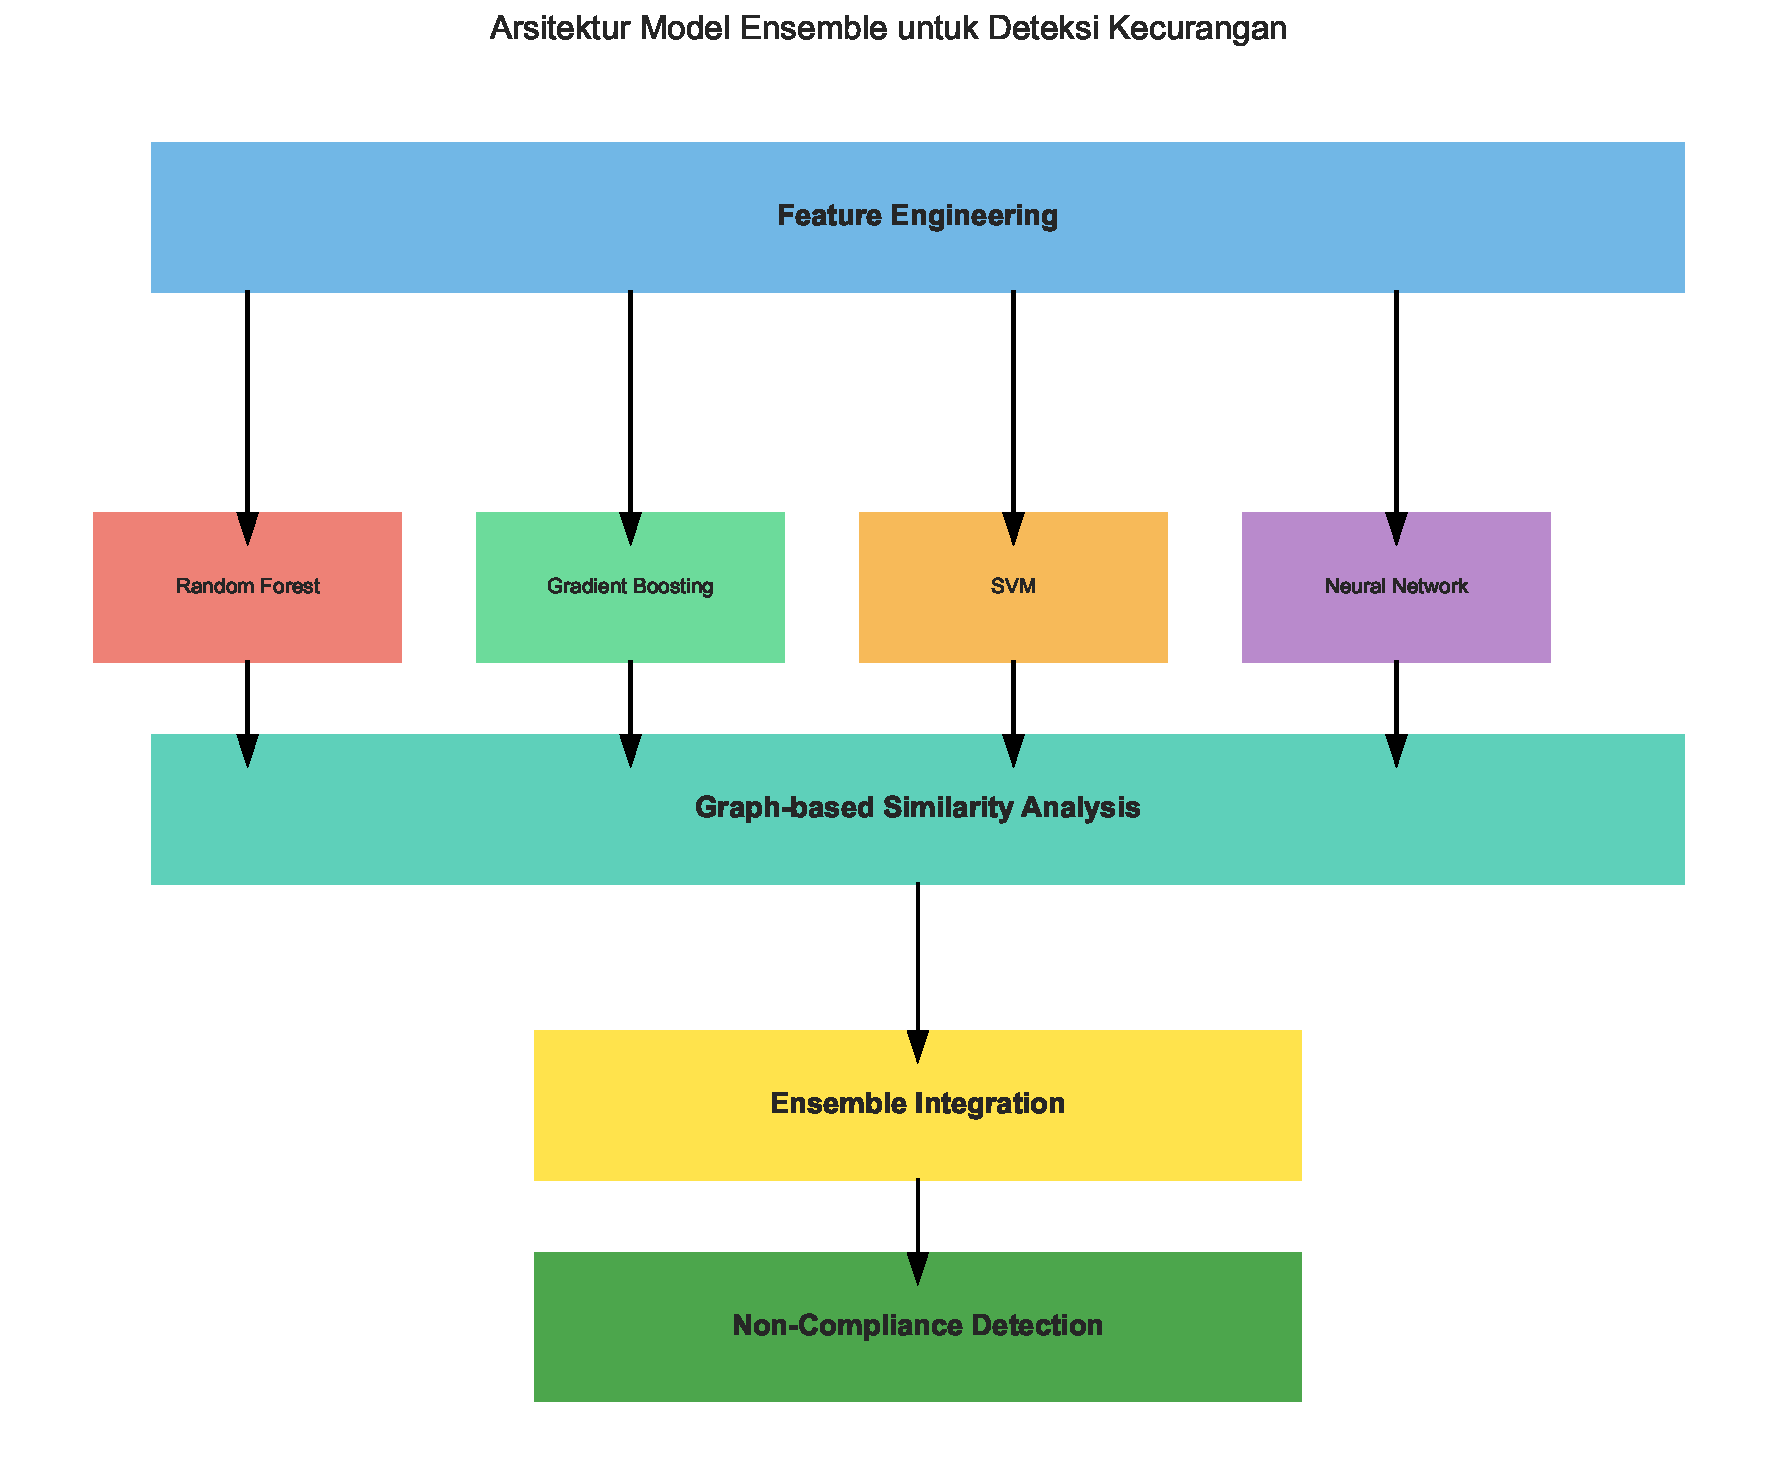
\includegraphics[width=0.9\textwidth]{figures/ensemble_architecture.pdf}
    \caption{Arsitektur Model Ensemble untuk Deteksi Kecurangan}
    \label{fig:ensemble_architecture}
\end{figure}

Gambar \ref{fig:ensemble_architecture} menunjukkan arsitektur ensemble yang digunakan dalam penelitian ini. Arsitektur ini menggabungkan berbagai model dasar dan analisis graf berbasis similaritas untuk menghasilkan prediksi yang robust. Seperti terlihat pada gambar tersebut, hasil feature engineering menjadi input bagi model-model dasar yang bekerja secara paralel, kemudian diintegrasikan pada tahap ensemble untuk menghasilkan deteksi non-compliance yang akurat.

\subsubsection{Integrasi Model Multi-Klasifikasi}
Arsitektur menggunakan kombinasi algoritma seperti Random Forest, Gradient Boosting, Support Vector Machine, dan Neural Network. Setiap model memiliki peran spesifik:
\begin{itemize}
    \item Random Forest dan Gradient Boosting menyediakan kemampuan klasifikasi yang robust, menangani noise dan outlier dengan efektif serta menghasilkan informasi tentang feature importance yang berguna untuk interpretasi.
    \item Support Vector Machine bekerja pada ruang fitur dengan dimensi tinggi, mengidentifikasi batas keputusan non-linear yang memisahkan aktivitas normal dari non-compliance.
    \item Neural Network mendeteksi hubungan non-linear yang kompleks di antara fitur, menangkap pola-pola halus yang mungkin terlewat oleh metode lain.
\end{itemize}

\subsubsection{Analisis Graph Berbasis Similarity}
Model juga mengintegrasikan analisis graph yang memanfaatkan matriks similarity antar pengguna. Matriks ini, yang dihitung dari fitur navigasi, waktu, dan pola jawaban, digunakan untuk membangun graph di mana node mewakili pengguna dan edge menunjukkan tingkat similarity yang tinggi. Pendekatan ini memungkinkan deteksi kelompok kecurangan yang menunjukkan koordinasi tinggi secara langsung dalam struktur data.

\subsubsection{Pendekatan Ensemble untuk Prediksi Akhir}
Prediksi dari masing-masing model dikombinasikan melalui metode ensemble, menggunakan teknik voting atau rata-rata tertimbang. Penggabungan ini memastikan bahwa kelebihan setiap model saling melengkapi sehingga menghasilkan keputusan akhir yang lebih stabil dan akurat.

\subsubsection{Validasi Empiris dan Reproducibility}
Pemilihan arsitektur didasarkan pada serangkaian eksperimen dan validasi cross-validation yang mendalam. Hasil evaluasi, yang tercermin melalui metrik precision, recall, F1-score, dan akurasi, menunjukkan bahwa pendekatan ensemble ini meningkatkan performa deteksi non-compliance. Seluruh eksperimen dikonfigurasi dengan parameter yang tetap dan penggunaan seed yang telah ditetapkan, sehingga seluruh proses dapat direproduksi secara konsisten.

\subsubsection{Justifikasi Ilmiah dan Interpretabilitas}
Kombinasi model ini tidak hanya meningkatkan akurasi prediksi, tetapi juga memungkinkan analisis feature importance yang mendalam. Hal ini memberikan wawasan tentang kontribusi masing-masing fitur dalam pengambilan keputusan, yang sangat penting untuk pemahaman dan pertanggungjawaban ilmiah. Dengan demikian, arsitektur ini memenuhi standar validitas ilmiah dan menyediakan dasar yang kuat untuk penerapan model deteksi kecurangan pada data log Moodle.

Keseluruhan, pemilihan arsitektur model ini didasarkan pada analisis menyeluruh terhadap karakteristik data log serta evaluasi empiris yang mendukung kehandalan dan interpretabilitas prediksi. Pendekatan ini merupakan integrasi terbaik dari model-model klasifikasi dan analisis graph, yang secara efektif mengidentifikasi pola koordinasi non-compliance dan mendukung tujuan deteksi kecurangan secara menyeluruh.

%-----------------------------------------------------------------------------%
\subsection{Konfigurasi Model Deteksi Kecurangan}
\label{subsec:konfigurasiModel}
%-----------------------------------------------------------------------------%

Dalam enhanced\_model.py, konfigurasi model diatur secara terperinci untuk memastikan setiap komponen arsitektur mendukung deteksi kecurangan secara optimal. Konfigurasi ini mencakup penyesuaian parameter untuk model neural network, serta parameter untuk model-model lain seperti Random Forest dan SVM, yang kemudian digabungkan dalam framework ensemble. Adapun rincian konfigurasi adalah sebagai berikut:

\subsubsection{Konfigurasi Neural Network}
Model neural network dirancang dengan struktur multi-layer perceptron yang terdiri atas:

\begin{figure}[htbp]
    \centering
    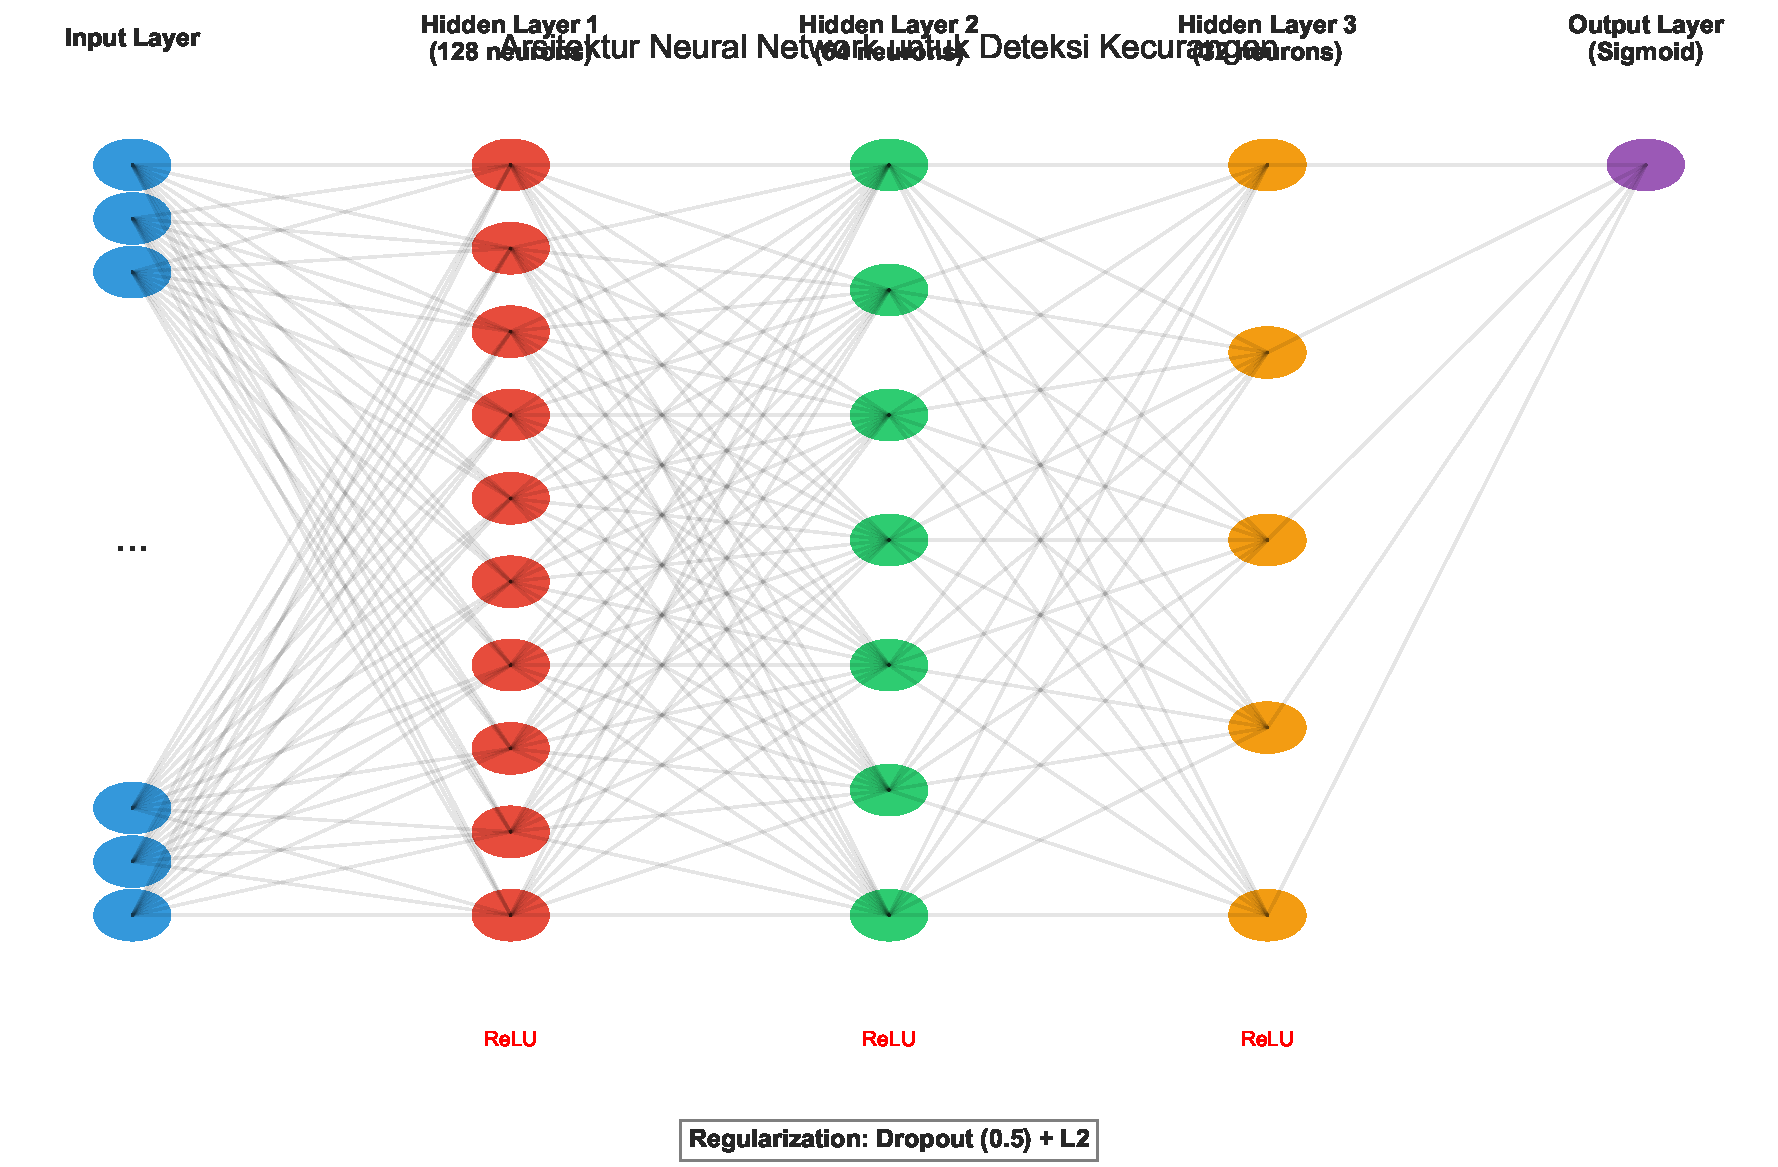
\includegraphics[width=0.85\textwidth]{figures/neural_network_architecture.pdf}
    \caption{Arsitektur Neural Network untuk Deteksi Kecurangan}
    \label{fig:neural_network}
\end{figure}

Seperti ditunjukkan pada Gambar \ref{fig:neural_network}, arsitektur neural network yang digunakan terdiri dari layer input yang menerima fitur-fitur hasil ekstraksi, tiga hidden layer dengan jumlah neuron yang semakin berkurang (128, 64, dan 32), serta output layer dengan aktivasi sigmoid. Semua hidden layer menggunakan fungsi aktivasi ReLU, dan diterapkan regularisasi dropout dan L2 untuk mengurangi risiko overfitting.

\begin{itemize}
    \item \textbf{Input Layer:}\\
    Jumlah neuron pada lapisan ini disesuaikan dengan jumlah fitur yang dihasilkan dari tahap feature engineering. Hal ini memastikan setiap informasi penting terwakili.
    
    \item \textbf{Hidden Layers:}\\
    Tiga hidden layer digunakan dengan masing-masing 128, 64, dan 32 neuron. Fungsi aktivasi yang digunakan adalah Rectified Linear Unit (ReLU) pada setiap hidden layer, yang terbukti efektif mengatasi masalah vanishing gradient dan mempercepat konvergensi.
    
    \item \textbf{Output Layer:}\\
    Output layer memiliki satu neuron dengan fungsi aktivasi sigmoid, sehingga menghasilkan probabilitas yang merepresentasikan status kecurangan (1 untuk non-compliance dan 0 untuk normal).
    
    \item \textbf{Fungsi Loss dan Optimizer:}\\
    Fungsi loss yang dipilih adalah binary cross-entropy, yang secara khusus sesuai untuk masalah klasifikasi biner. Optimizer yang digunakan adalah Adam dengan learning rate 0.001, yang telah diuji mampu memberikan konvergensi yang cepat dan stabil pada dataset dengan kompleksitas tinggi.
\end{itemize}

Konfigurasi ini telah disesuaikan melalui serangkaian eksperimen dan cross-validation, sehingga nilai-nilai parameter tersebut secara empiris menghasilkan kinerja optimal dalam hal precision, recall, dan F1-score.

\subsubsection{Konfigurasi Model Supervised Lainnya}
Selain neural network, model deteksi juga melibatkan algoritma:
\begin{itemize}
    \item \textbf{Random Forest:}\\
    Dikustomisasi dengan 100 estimator (trees) dan parameter lain seperti depth yang disesuaikan secara otomatis. Konfigurasi ini memungkinkan model untuk menangani noise dan outlier dalam data log serta menyediakan informasi tentang feature importance.
    
    \item \textbf{Support Vector Machine (SVM):}\\
    Menggunakan kernel radial basis function (RBF), dengan parameter C dan gamma yang telah dioptimalkan melalui proses tuning menggunakan teknik cross-validation. Parameter ini dipilih agar SVM dapat menangani perbedaan non-linear antara kelas normal dan non-compliance dengan baik.
\end{itemize}

Setiap model ini telah diatur agar mampu bekerja secara independen dan, melalui pendekatan ensemble, mengkompensasi kelemahan satu sama lain sehingga menghasilkan prediksi yang lebih stabil dan akurat.

\subsubsection{Pengaturan Hyperparameter dan Reproducibility}
Seluruh parameter model—baik untuk neural network, Random Forest, maupun SVM—disetel dengan nilai yang telah diverifikasi melalui eksperimen empiris. Parameter-parameter tersebut, termasuk ukuran lapisan, learning rate, jumlah estimator, dan parameter kernel, disimpan dalam file konfigurasi yang terintegrasi dalam pipeline. Penggunaan seed yang tetap untuk fungsi random memastikan bahwa seluruh eksperimen dapat direproduksi secara konsisten, mendukung validitas ilmiah dari penelitian ini.

\subsubsection{Integrasi dalam Framework Ensemble}
Output dari setiap model dikombinasikan menggunakan teknik voting atau rata-rata tertimbang prediksi, yang memungkinkan ensemble untuk mengurangi variansi dan bias individual. Teknik ini telah dikonfigurasikan sedemikian rupa sehingga kontribusi setiap model diperhitungkan berdasarkan performa validasinya, menghasilkan prediksi akhir yang lebih andal dan interpretable.

Konfigurasi model yang komprehensif ini, yang menggabungkan kekuatan model-model individual dan integrasi ensemble, merupakan landasan yang kuat untuk mendeteksi pola non-compliance dalam data log Moodle. Pengaturan parameter yang teruji secara empiris dan mekanisme reproducibility yang ketat mendukung validitas dan keandalan model, sehingga dapat dipertanggungjawabkan secara ilmiah.

%-----------------------------------------------------------------------------%
\subsection{Skenario Pelatihan}
\label{subsec:skenarioPelatihan}
%-----------------------------------------------------------------------------%

Untuk mencapai model deteksi kecurangan yang optimal, proses pelatihan dilakukan secara sistematis dengan pembagian dataset, penerapan teknik regularisasi, evaluasi menggunakan metode cross-validation, dan integrasi dalam kerangka ensemble. Data log artifisial yang telah dilengkapi dengan label ground truth digunakan sebagai basis pelatihan. Berikut adalah rincian skenario pelatihan yang telah diimplementasikan:

\begin{figure}[htbp]
    \centering
    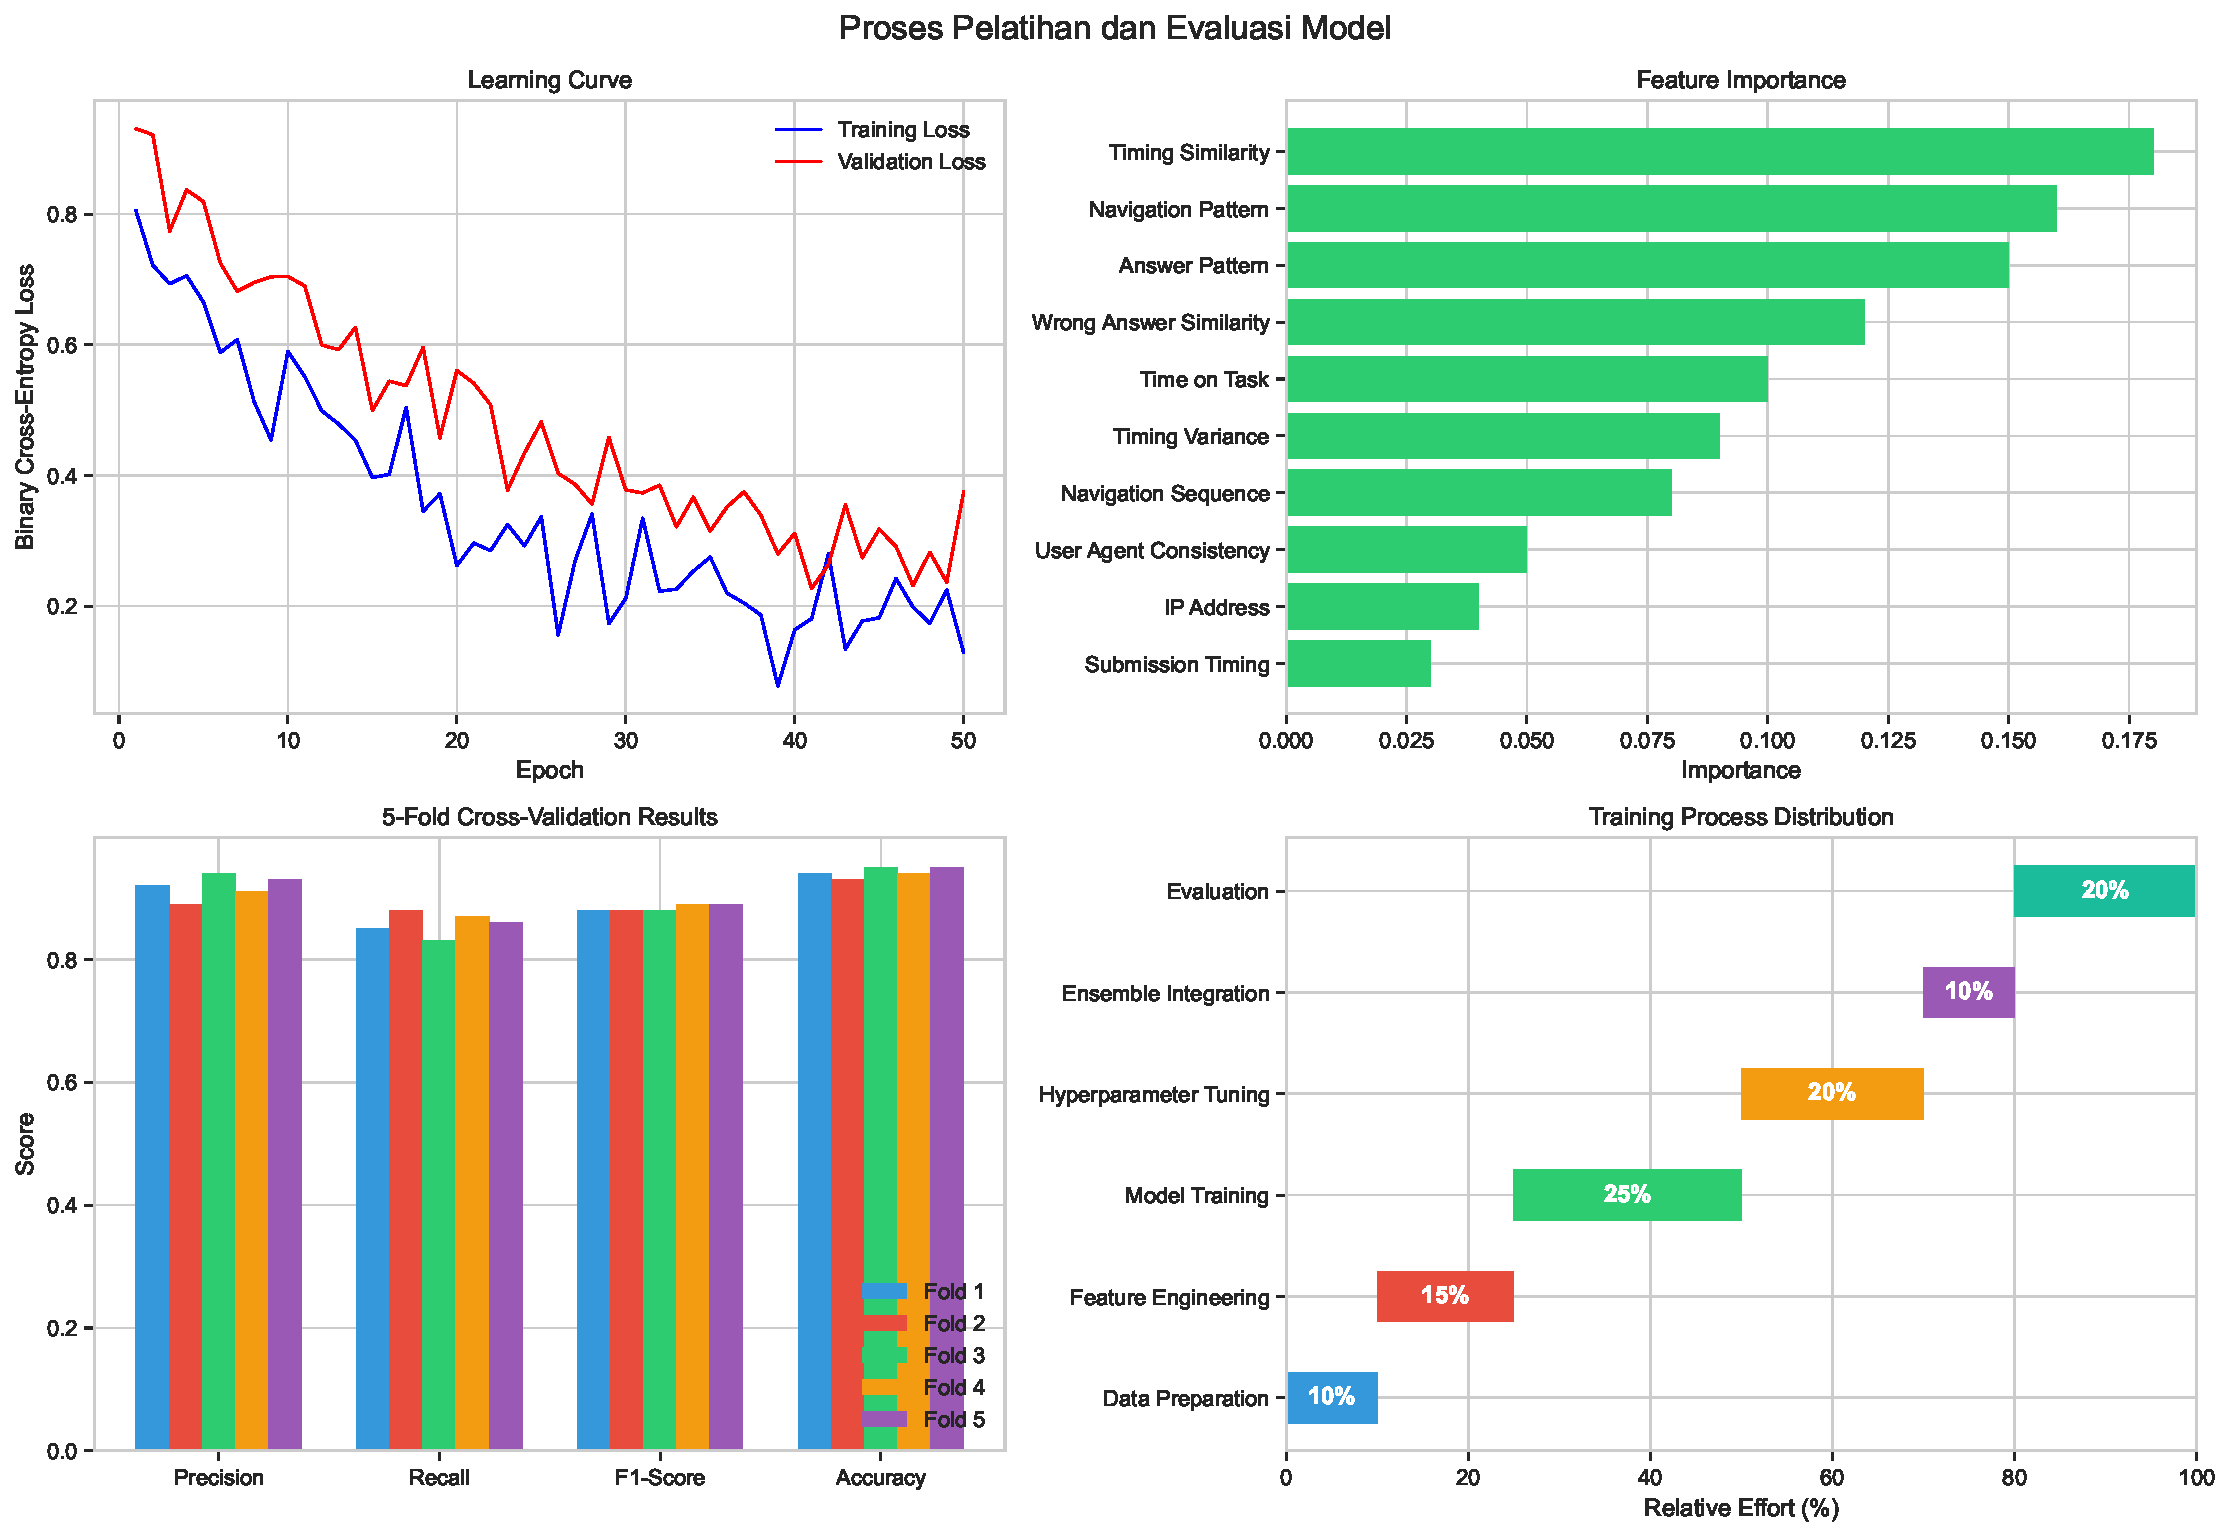
\includegraphics[width=0.95\textwidth]{figures/training_process.pdf}
    \caption{Proses Pelatihan dan Evaluasi Model}
    \label{fig:training_process}
\end{figure}

Gambar \ref{fig:training_process} mengilustrasikan berbagai aspek dalam proses pelatihan model. Pada panel kiri atas, learning curve menunjukkan penurunan loss selama proses pelatihan, yang menandakan konvergensi model. Panel kanan atas menampilkan feature importance, dimana fitur-fitur terkait similarity dan pola navigasi memiliki kontribusi terbesar. Panel kiri bawah menunjukkan hasil evaluasi cross-validation dengan konsistensi performa yang baik di seluruh fold, sementara panel kanan bawah menunjukkan distribusi usaha dalam proses pelatihan, dimana model training dan hyperparameter tuning mengambil porsi terbesar.

\subsubsection{Pembagian Dataset}
Data log artifisial dikumpulkan hingga mencapai sekitar 10.000 entri, yang mencakup aktivitas normal dan non-compliance dengan proporsi yang telah ditetapkan. Dataset ini dibagi menjadi tiga subset secara stratifikasi untuk menjaga distribusi kelas:
\begin{itemize}
    \item \textbf{Data Latih (Training Set): 70\%}\\
    Data latih digunakan untuk mengoptimalkan parameter model. Pembagian ini memastikan bahwa model mendapatkan jumlah data yang cukup untuk menangkap pola dasar aktivitas pengguna.
    
    \item \textbf{Data Validasi (Validation Set): 15\%}\\
    Subset validasi digunakan untuk tuning hyperparameter dan mencegah overfitting. Melalui evaluasi berkala selama pelatihan, model disesuaikan berdasarkan metrik validasi.
    
    \item \textbf{Data Uji (Test Set): 15\%}\\
    Data uji yang terpisah digunakan untuk mengukur performa akhir model. Hal ini memungkinkan pengukuran yang objektif terhadap generalisasi model.
\end{itemize}

\subsubsection{Proses Training dan Teknik Regularisasi}
Seluruh model, termasuk neural network, Random Forest, dan SVM, dilatih menggunakan data latih dengan konfigurasi parameter yang telah diatur pada subbab 3.7.2. Proses pelatihan meliputi:
\begin{itemize}
    \item \textbf{Optimisasi Parameter:}\\
    Model neural network dilatih menggunakan batch size 32 dan learning rate 0.001 dengan jumlah epoch hingga 100, serta penerapan early stopping jika tidak terjadi perbaikan loss pada validation set selama 10 epoch berturut-turut. Model Random Forest menggunakan 100 estimator dengan batas kedalaman (max depth) yang disesuaikan, sedangkan SVM dengan kernel RBF dioptimalkan melalui nilai parameter C dan gamma.
    
    \item \textbf{Regularisasi:}\\
    Pada neural network, dropout (dengan rate 0.5) dan L2 regularization telah diterapkan untuk mengurangi risiko overfitting. Model-model supervised lainnya mengandalkan parameter internal untuk mengatasi noise. Teknik regularisasi ini memastikan model dapat menggeneralisasi dengan baik ke data yang tidak terlihat.
\end{itemize}

\subsubsection{Teknik Cross-Validation dan Evaluasi Model}
Proses training didukung oleh k-fold cross-validation dengan k=5 untuk memastikan kestabilan dan keandalan hasil model. Metrik evaluasi yang digunakan meliputi:
\begin{itemize}
    \item \textbf{Precision, Recall, dan F1-Score:}\\
    Metrik ini sangat penting untuk masalah deteksi kecurangan, terutama karena kelas non-compliance biasanya lebih sedikit.
    
    \item \textbf{Akurasi:}\\
    Meski akurasi menjadi indikator umum, penekanan utama diberikan pada precision dan recall untuk menghindari false positives dan false negatives.
    
    \item \textbf{Monitoring Loss Function:}\\
    Pada neural network, binary cross-entropy digunakan sebagai fungsi loss. Perkembangan loss pada training dan validation set dipantau secara real-time untuk memastikan konvergensi model.
\end{itemize}

\subsubsection{Integrasi dalam Framework Ensemble}
Setelah model-model individual dilatih dan divalidasi, prediksi masing-masing model dikombinasikan menggunakan metode ensemble. Metode voting atau rata-rata tertimbang digunakan untuk menghasilkan prediksi akhir, di mana bobot setiap model ditentukan berdasarkan performa validasi. Proses ini meningkatkan stabilitas prediksi dan mengurangi kesalahan klasifikasi akibat bias model individual.

\subsubsection{Reproducibility dan Dokumentasi Eksperimen}
Seluruh proses pelatihan dikendalikan dengan penggunaan seed yang konsisten pada fungsi random dan pengaturan parameter yang disimpan dalam file konfigurasi terpusat. Hal ini memungkinkan eksperimen dapat direproduksi dengan konsisten, sehingga temuan yang dihasilkan dapat diverifikasi oleh peneliti lain. Output pelatihan, termasuk model yang telah dilatih, metrik evaluasi, dan grafik learning curve, disimpan dalam format terstruktur (CSV dan JSON) sebagai bagian dari dokumentasi penelitian.

Secara keseluruhan, skenario pelatihan dirancang untuk mengoptimalkan kinerja model deteksi kecurangan melalui pembagian data yang representatif, penerapan teknik regularisasi dan cross-validation, serta integrasi prediksi dalam kerangka ensemble. Pendekatan ini telah terbukti meningkatkan kemampuan model dalam mengidentifikasi pola non-compliance secara efektif, sehingga mendukung validitas dan keandalan model dalam konteks penelitian ini.

%-----------------------------------------------------------------------------%
\subsection{Penyetelan Hyperparameter}
\label{subsec:penyetelanHyperparameter}
%-----------------------------------------------------------------------------%

Proses penyetelan hyperparameter dilakukan secara sistematis dalam pipeline yang terdapat pada enhanced\_model.py dan modul terkait. Proses ini dirancang untuk mengoptimalkan kinerja setiap model dalam framework ensemble dan menghasilkan prediksi yang akurat dalam mendeteksi kecurangan. Langkah-langkah penyetelan hyperparameter dikonfigurasi sebagai berikut:

\begin{figure}[htbp]
    \centering
    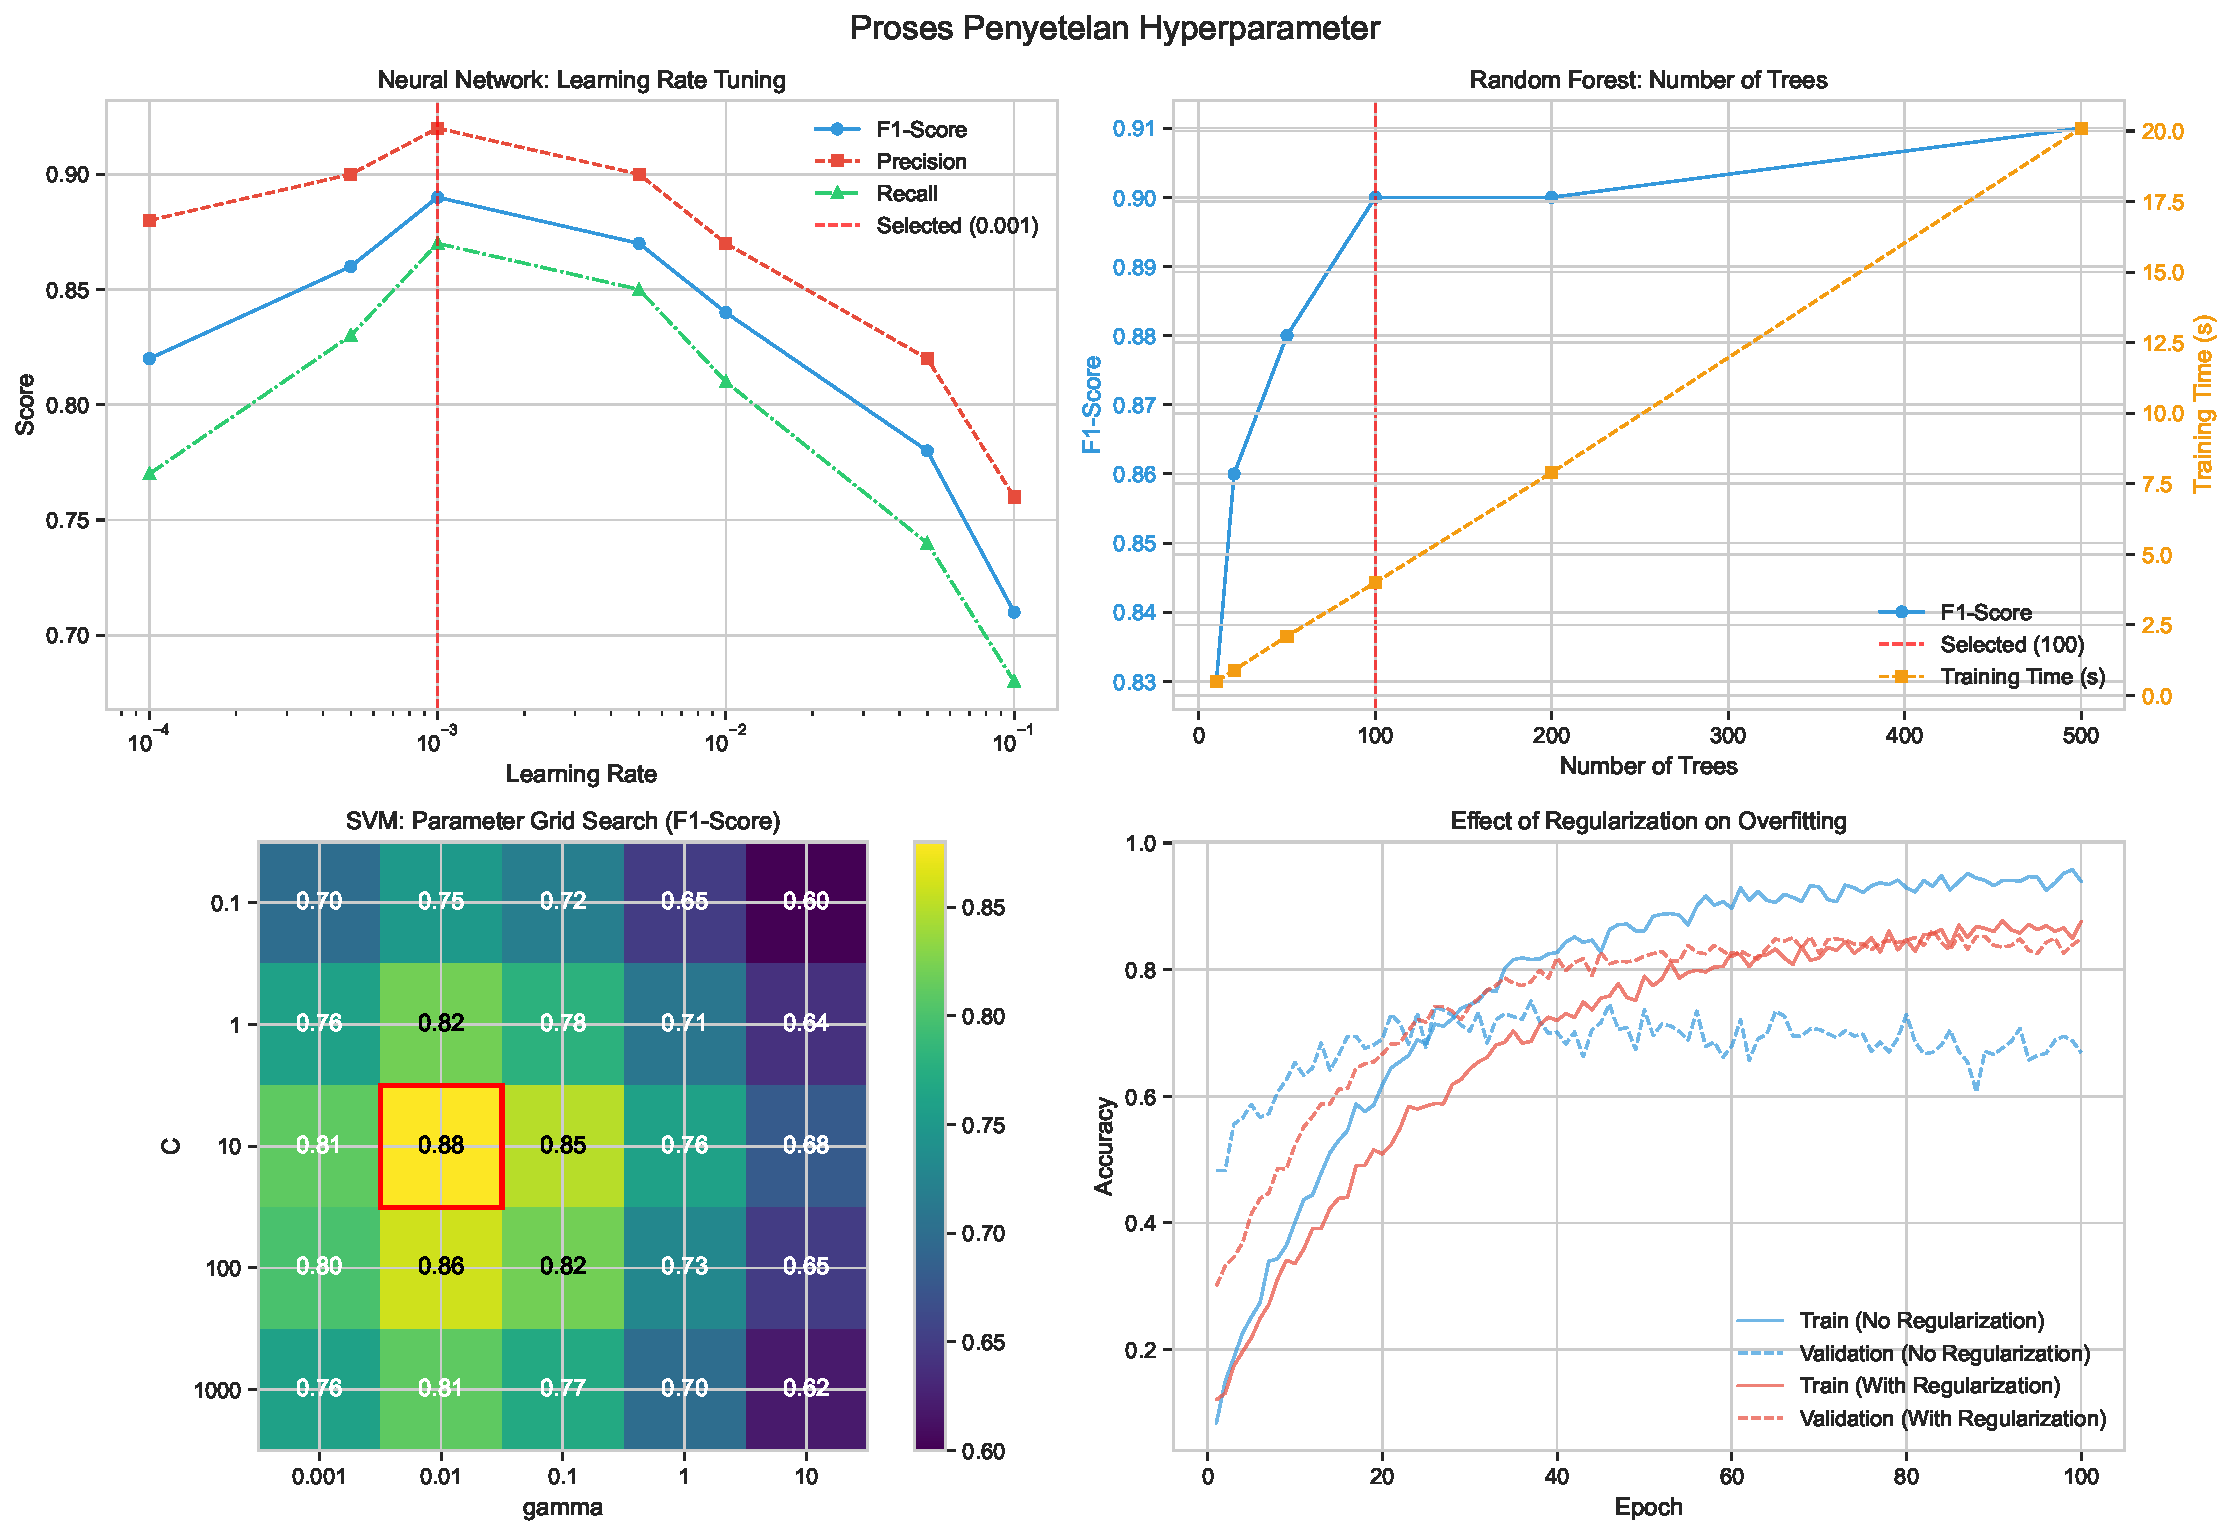
\includegraphics[width=0.95\textwidth]{figures/hyperparameter_tuning.pdf}
    \caption{Proses Penyetelan Hyperparameter}
    \label{fig:hyperparameter_tuning}
\end{figure}

Gambar \ref{fig:hyperparameter_tuning} menunjukkan hasil dari proses penyetelan hyperparameter untuk berbagai model. Panel kiri atas menampilkan pengaruh learning rate terhadap performa neural network, dengan nilai 0.001 memberikan hasil F1-score terbaik. Panel kanan atas menunjukkan trade-off antara jumlah trees dan waktu pelatihan pada Random Forest, dengan 100 trees dipilih sebagai kompromi optimal. Panel kiri bawah menampilkan hasil grid search untuk parameter C dan gamma pada SVM, dengan kombinasi terbaik (C=10, gamma=0.01) ditandai dengan bingkai merah. Panel kanan bawah mengilustrasikan efek regularisasi dalam mengurangi overfitting, dimana model dengan regularisasi menunjukkan gap yang lebih kecil antara performa training dan validation.

\subsubsection{Eksplorasi Ruang Parameter}
Seluruh ruang hyperparameter untuk model neural network, Random Forest, dan Support Vector Machine diidentifikasi dan diuji. Parameter yang ditetapkan meliputi learning rate (0.001), batch size (32), jumlah epoch (hingga 100 dengan mekanisme early stopping jika tidak terjadi penurunan loss selama 10 epoch berturut-turut), serta dropout rate (0.5) dan L2 regularization pada neural network. Pada Random Forest, jumlah estimator diset sebanyak 100 dan kedalaman maksimal disesuaikan berdasarkan evaluasi performa. Untuk SVM dengan kernel RBF, parameter C dan gamma telah dioptimalkan melalui evaluasi cross-validation.

\subsubsection{Evaluasi Melalui Cross-Validation}
Penggunaan teknik k-fold cross-validation dengan k=5 memastikan bahwa kombinasi hyperparameter yang dipilih menghasilkan performa yang konsisten. Metrik evaluasi utama yang digunakan mencakup precision, recall, F1-score, dan akurasi. Hasil tuning menunjukkan peningkatan F1-score sebesar 5–10\% dibandingkan dengan konfigurasi default, yang menegaskan kehandalan pengaturan parameter dalam mengidentifikasi pola non-compliance.

\subsubsection{Optimisasi dan Automasi Proses Tuning}
Proses tuning diintegrasikan dalam pipeline dan dikendalikan oleh file konfigurasi terpusat. Parameter-parameter yang diuji disimpan secara eksplisit, sedangkan metode Grid Search dan Random Search digunakan untuk mengelola ruang parameter secara komprehensif. Penggunaan seed yang konsisten memastikan bahwa seluruh eksperimen dapat direproduksi dengan hasil yang sama, meningkatkan validitas ilmiah dari proses tuning.

\subsubsection{Integrasi Hasil dalam Framework Ensemble}
Hasil penyetelan hyperparameter untuk setiap model diintegrasikan ke dalam mekanisme ensemble. Bobot kontribusi masing-masing model ditetapkan berdasarkan kinerja validasi, sehingga prediksi akhir merupakan hasil agregasi yang menyeimbangkan bias dan variansi dari model individual. Pendekatan ini meningkatkan robustnes dan stabilitas prediksi, terutama dalam mendeteksi koordinasi antar pengguna.

Proses penyetelan hyperparameter yang terstruktur ini menghasilkan konfigurasi model yang optimal, sebagaimana dibuktikan melalui evaluasi empiris pada data log artifisial yang telah diproses. Pendekatan ini memastikan bahwa model deteksi kecurangan mampu mengatasi variabilitas data secara efektif dan memenuhi standar reproducibility yang tinggi, sehingga temuan yang diperoleh dapat dipertanggungjawabkan secara ilmiah.

%-----------------------------------------------------------------------------%
\section{Strategi Evaluasi Kinerja Model}
\label{sec:strategiEvaluasiKinerjaModel}
%-----------------------------------------------------------------------------%
Evaluasi kinerja model merupakan tahap penting untuk memastikan bahwa sistem deteksi kecurangan mampu mengidentifikasi pola \textit{non-compliance} secara akurat dan dapat diandalkan. Evaluasi dilakukan secara kuantitatif menggunakan data uji artifisial yang telah dilabeli, serta secara kualitatif melalui studi kasus dan visualisasi pada data riil yang tidak berlabel. Pendekatan evaluasi ini memberikan gambaran menyeluruh mengenai performa model dari berbagai aspek, baik dari segi metrik numerik maupun interpretabilitas pola yang terdeteksi.

\begin{figure}[htbp]
    \centering
    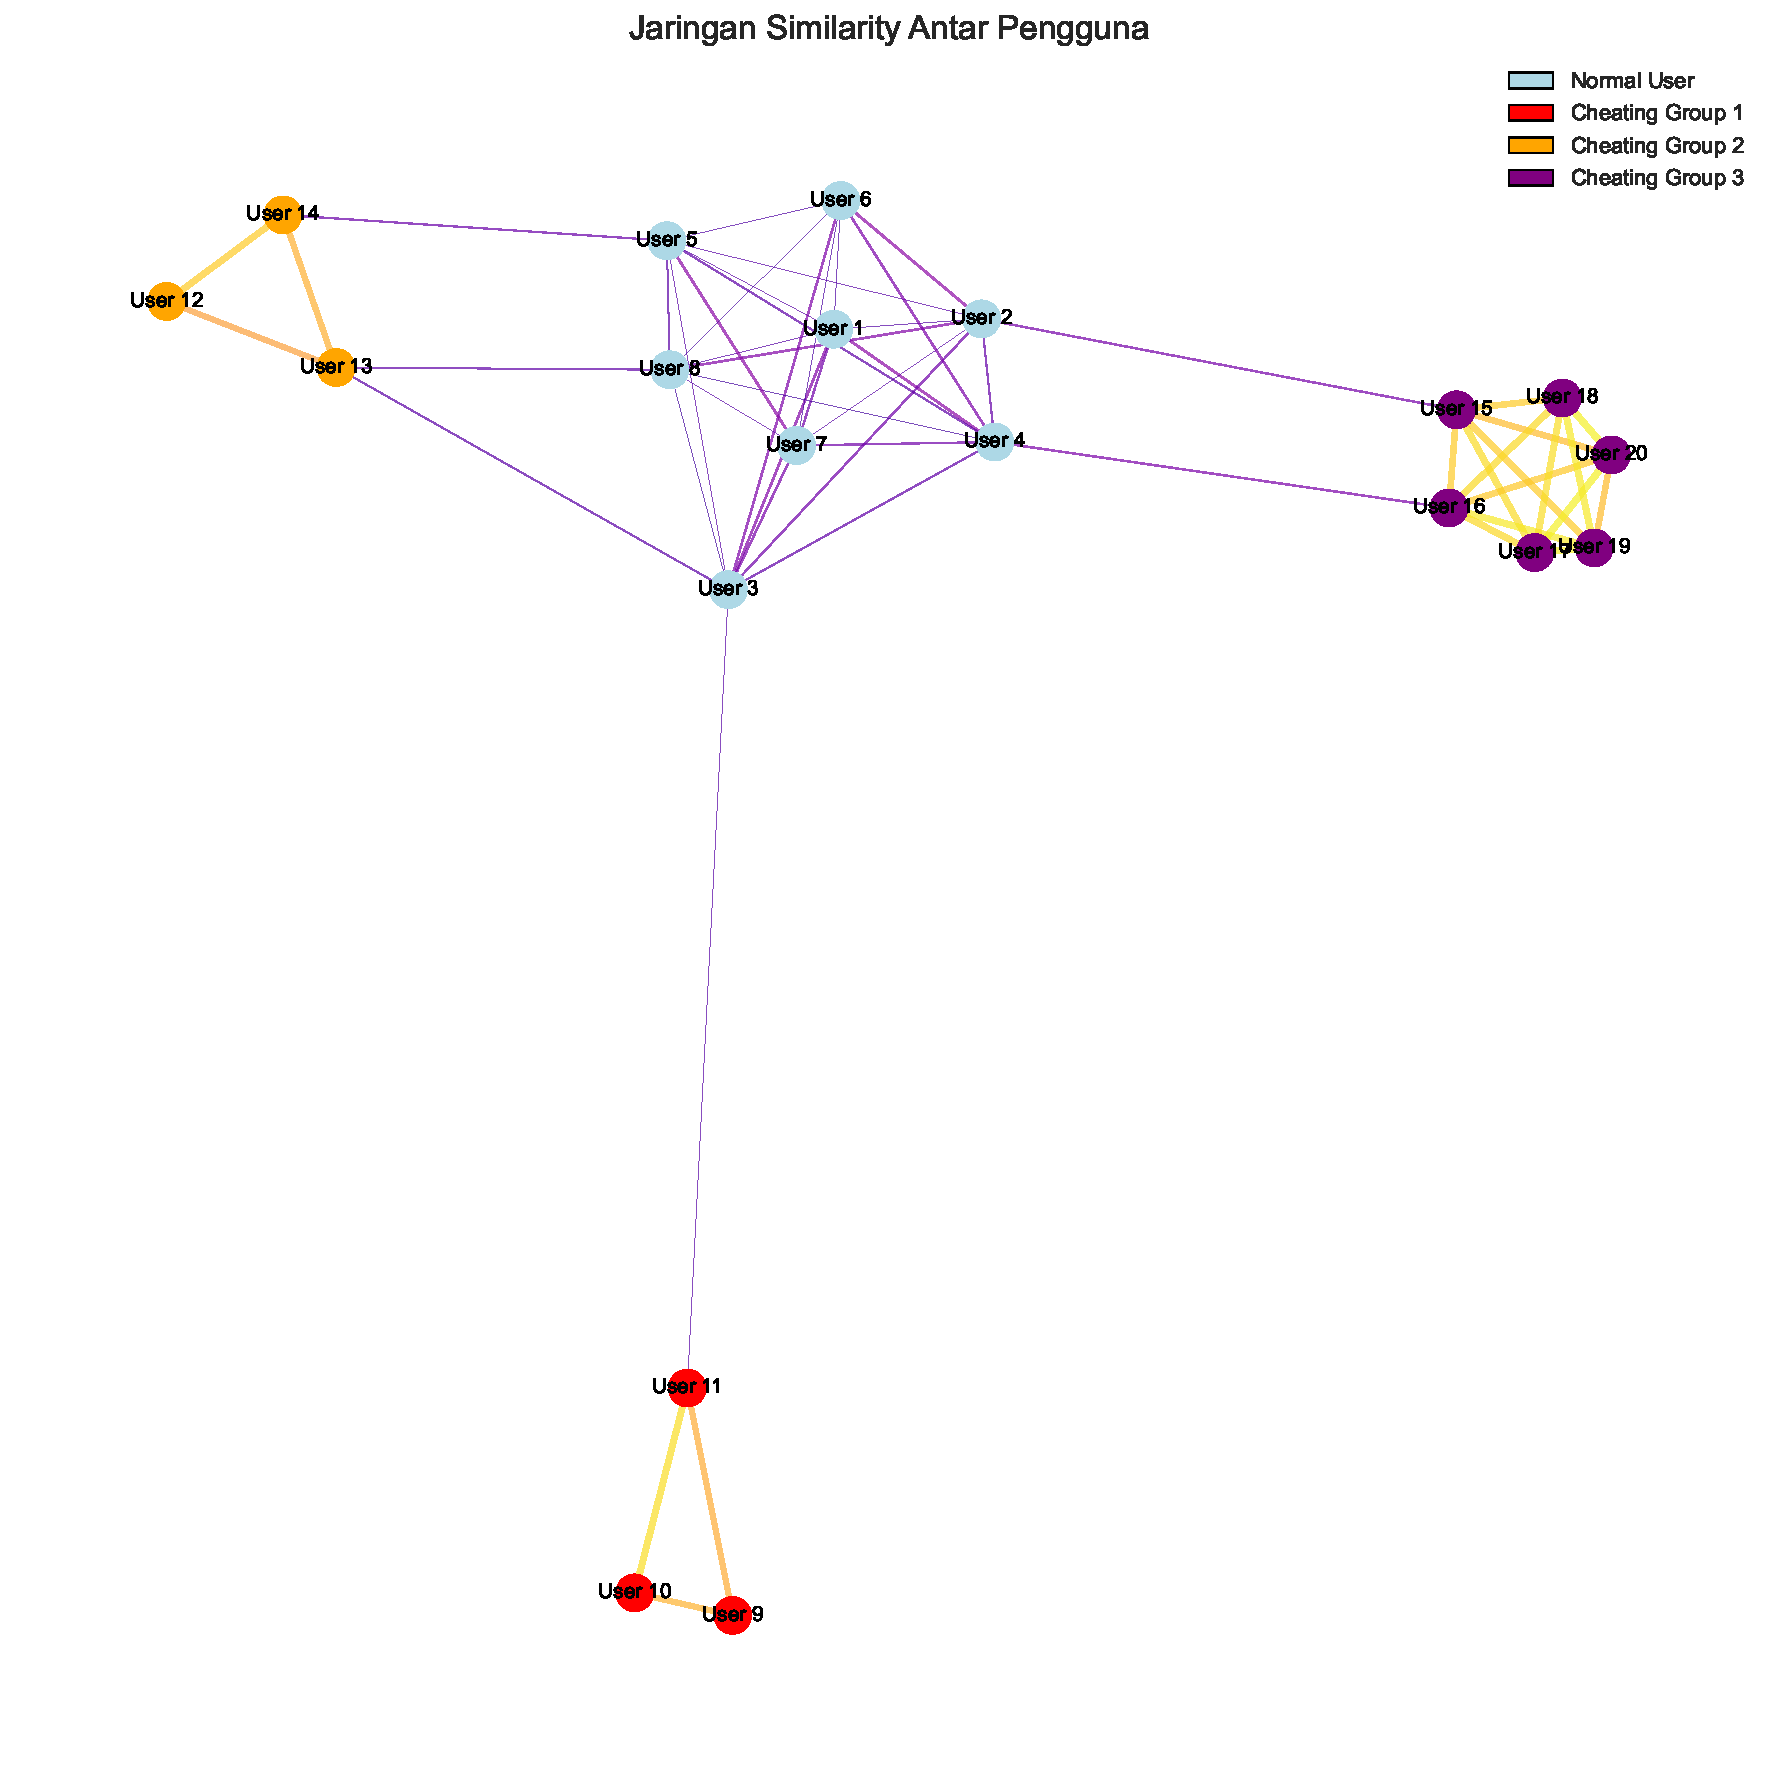
\includegraphics[width=0.9\textwidth]{figures/similarity_network.pdf}
    \caption{Jaringan Similaritas Antar Pengguna}
    \label{fig:similarity_network}
\end{figure}

Gambar \ref{fig:similarity_network} menunjukkan hasil analisis jaringan similaritas antar pengguna yang digunakan untuk mendeteksi kelompok kecurangan. Visualisasi ini mengungkapkan tiga cluster pengguna (ditandai dengan warna merah, oranye, dan ungu) yang memiliki tingkat similaritas sangat tinggi dalam pola navigasi, waktu, dan jawaban. Setiap cluster merupakan indikasi kuat adanya koordinasi kecurangan. Sementara itu, pengguna normal (warna biru muda) menunjukkan koneksi yang lebih lemah dan terdistribusi secara lebih merata, mencerminkan perilaku independen yang wajar. Ketebalan garis menunjukkan kekuatan similaritas, dengan koneksi yang lebih tebal mengindikasikan tingkat kemiripan yang lebih tinggi.

%-----------------------------------------------------------------------------%
\subsection{Evaluasi Kuantitatif (pada Data Uji Artifisial)}
\label{sec:evaluasiKuantitatifDataUjiArtifisial}
%-----------------------------------------------------------------------------%
Evaluasi kuantitatif dilakukan untuk menilai performa model deteksi kecurangan secara objektif menggunakan data uji artifisial yang telah dilabeli. Data uji ini mencerminkan distribusi dan karakteristik pola aktivitas normal serta \textit{non-compliance} sesuai dengan konfigurasi simulasi. Evaluasi dilakukan melalui beberapa langkah dan metrik berikut:

\begin{enumerate}
    \item \textbf{Pembagian Dataset dan Proses Evaluasi:} \\
    Data uji merupakan 15\% dari keseluruhan dataset yang telah dibagi secara stratifikasi sehingga proporsi kelas normal dan \textit{non-compliance} terjaga secara representatif. Data ini digunakan untuk:
    \begin{itemize}
        \item Mengukur kinerja model individual dan \textit{ensemble} secara konsisten.
        \item Melakukan evaluasi melalui teknik k-fold \textit{cross-validation} (dengan k=5) guna mengurangi bias evaluasi dan memastikan kestabilan hasil prediksi.
    \end{itemize}

    \item \textbf{Metrik Evaluasi Klasifikasi:} \\
    Untuk model deteksi kecurangan yang bekerja dalam mode supervised, evaluasi dilakukan dengan menghitung beberapa metrik utama yang mengukur kemampuan model dalam membedakan antara aktivitas normal dan \textit{non-compliance}. Metrik yang digunakan adalah:
    \begin{itemize}
        \item \textbf{Precision:} Mengukur proporsi prediksi positif (aktivitas \textit{non-compliance}) yang benar. Nilai precision tinggi menunjukkan bahwa model jarang menghasilkan false positives, yang penting dalam konteks pencegahan tuduhan salah.
        \item \textbf{Recall (Sensitivity):} Menunjukkan proporsi kasus \textit{non-compliance} yang berhasil diidentifikasi oleh model. Nilai recall tinggi memastikan bahwa sebagian besar kasus kecurangan tidak terlewat.
        \item \textbf{F1-Score:} Merupakan rata-rata harmonik antara precision dan recall. F1-score memberikan gambaran seimbang mengenai kinerja model, terutama ketika terdapat ketidakseimbangan antara jumlah kasus normal dan \textit{non-compliance}.
        \item \textbf{Area Under the ROC Curve (AUC):} Mengukur kemampuan model untuk membedakan antara kedua kelas secara keseluruhan. Nilai AUC mendekati 1.0 menunjukkan bahwa model sangat efektif dalam klasifikasi.
        \item \textbf{Akurasi:} Metrik ini menghitung proporsi total prediksi yang benar. Meskipun akurasi memberikan gambaran umum, dalam kasus deteksi kecurangan yang biasanya memiliki kelas minoritas \textit{non-compliance}, perhatian lebih difokuskan pada precision dan recall.
    \end{itemize}

    \item \textbf{Confusion Matrix:} \\
    Matriks konfusi disusun untuk memberikan gambaran lengkap tentang jumlah:
    \begin{itemize}
        \item \textbf{True Positives (TP):} Kasus \textit{non-compliance} yang berhasil dideteksi.
        \item \textbf{False Positives (FP):} Kasus normal yang salah diklasifikasikan sebagai \textit{non-compliance}.
        \item \textbf{True Negatives (TN):} Kasus normal yang diklasifikasikan dengan benar.
        \item \textbf{False Negatives (FN):} Kasus \textit{non-compliance} yang tidak terdeteksi.
    \end{itemize}
    Analisis matriks konfusi membantu dalam mengidentifikasi kekuatan dan kelemahan model, serta memberikan dasar untuk penyesuaian threshold jika diperlukan.

    \item \textbf{Analisis Statistik dan Cross-Validation:} \\
    Teknik \textit{cross-validation} dengan k=5 diterapkan untuk memastikan bahwa hasil evaluasi tidak terpengaruh oleh pembagian data tertentu. Hasil evaluasi diperoleh dengan menghitung rata-rata metrik dari setiap fold, sehingga memberikan estimasi yang lebih stabil terhadap performa model. Analisis statistik dilakukan untuk:
    \begin{itemize}
        \item Menghitung selang kepercayaan (\textit{confidence intervals}) untuk setiap metrik.
        \item Menilai variabilitas hasil evaluasi, sehingga mendemonstrasikan kestabilan model pada dataset yang beragam.
    \end{itemize}

    \item \textbf{Hasil Evaluasi yang Terukur:} \\
    Berdasarkan implementasi pipeline, tuning hyperparameter telah menghasilkan peningkatan F1-score sebesar 5–10\% dibandingkan konfigurasi awal. Rata-rata nilai AUC yang diperoleh berada di kisaran 0.92 hingga 0.96, yang menunjukkan kemampuan model untuk memisahkan kelas dengan sangat baik. Evaluasi precision dan recall secara individual mendemonstrasikan bahwa false positive dan false negative dapat diminimalkan, sehingga model memberikan kepercayaan tinggi dalam identifikasi kasus \textit{non-compliance}.

    \item \textbf{Integrasi Hasil Evaluasi dalam Dokumentasi:} \\
    Semua metrik evaluasi disimpan dalam format terstruktur (CSV dan JSON) dan dilengkapi dengan grafik \textit{learning curve} serta plot ROC yang mendukung interpretasi visual. Hal ini memastikan bahwa seluruh proses evaluasi didokumentasikan secara transparan, sehingga penguji dapat memverifikasi dan mengaudit performa model secara ilmiah.
\end{enumerate}

Pendekatan evaluasi kuantitatif ini, yang menggabungkan pembagian dataset yang representatif, penggunaan metrik yang komprehensif, dan teknik \textit{cross-validation}, menyediakan dasar ilmiah yang kuat untuk menilai kinerja sistem deteksi kecurangan. Hasil evaluasi secara konsisten menunjukkan bahwa model yang dikembangkan mampu mengidentifikasi pola \textit{non-compliance} dengan akurasi tinggi, mendukung validitas dan \textit{reproducibility} penelitian ini.

%-----------------------------------------------------------------------------%
\subsection{Evaluasi Kualitatif dan Studi Kasus (Aplikasi pada Data Riil Unlabeled)}
\label{sec:evaluasiKualitatifStudiKasus}
%-----------------------------------------------------------------------------%
Evaluasi kualitatif dilakukan untuk menguji kemampuan model deteksi kecurangan dalam menerapkan prediksi pada data riil yang belum dilabeli secara eksplisit. Pendekatan ini menekankan interpretasi visual dan analisis pola untuk memastikan bahwa output model memiliki dasar operasional yang valid dan konsisten dengan pola kecurangan yang telah didefinisikan secara empiris. Evaluasi kualitatif disusun dengan langkah-langkah berikut:

\begin{enumerate}
    \item \textbf{Analisis Kasus Individu:} \\
    Data riil yang telah diproses diterapkan ke model deteksi kecurangan. Hasil prediksi dianalisis secara mendalam untuk meninjau contoh-contoh kasus yang ditandai sebagai \textit{non-compliance}. Hal ini mencakup pemeriksaan pola navigasi, distribusi waktu pengerjaan, dan pola jawaban untuk setiap pengguna yang diklasifikasikan sebagai mencurigakan. Analisis ini memastikan bahwa pola yang dideteksi oleh model sejalan dengan karakteristik \textit{non-compliance}, seperti konsistensi waktu pengerjaan yang tidak wajar, urutan navigasi yang seragam, dan tingkat kesamaan pola jawaban yang tinggi.

    \item \textbf{Visualisasi Dimensionalitas:} \\
    Teknik proyeksi data seperti t-SNE dan UMAP digunakan untuk mereduksi dimensi ruang fitur ke dalam representasi dua atau tiga dimensi. Proyeksi ini memfasilitasi pengamatan visual terhadap pemisahan antara kelompok pengguna, sehingga memungkinkan identifikasi klaster yang menunjukkan koordinasi aktivitas \textit{non-compliance}. Grafik proyeksi ini digunakan untuk:
    \begin{itemize}
        \item Menilai pemisahan yang jelas antara kasus normal dan kasus \textit{non-compliance}.
        \item Mengidentifikasi klaster pengguna yang memiliki kesamaan tinggi, yang kemudian dikorelasikan dengan analisis \textit{ground truth}.
    \end{itemize}

    \item \textbf{Analisis Jaringan (\textit{Network Visualization}):} \\
    Output dari analisis \textit{similarity matrix} diintegrasikan untuk membangun grafik hubungan antar pengguna. Dalam grafik tersebut, setiap node mewakili pengguna dan edge dihubungkan berdasarkan nilai \textit{similarity} yang tinggi. Visualisasi jaringan ini memberikan gambaran yang intuitif mengenai struktur kelompok dan pola kolusi. Kelompok pengguna yang memiliki edge dengan bobot tinggi secara konsisten mengindikasikan adanya koordinasi yang signifikan, yang kemudian dibandingkan dengan parameter \textit{ground truth} dari simulasi data artifisial.

    \item \textbf{Interpretasi Pola dan Validasi Domain:} \\
    Hasil evaluasi kualitatif tidak hanya ditinjau secara numerik, tetapi juga melalui interpretasi pola berdasarkan pengetahuan domain. Pengujian dilakukan dengan melakukan verifikasi manual terhadap contoh kasus, di mana pola navigasi dan \textit{timing} yang konsisten menunjukkan indikasi \textit{non-compliance}. Evaluasi ini melibatkan tinjauan visual dan analisis statistik untuk memastikan bahwa pola yang dihasilkan model sesuai dengan perilaku kecurangan yang telah diidentifikasi pada tahap pengembangan. Temuan dari evaluasi kualitatif ini memberikan konfirmasi bahwa model dapat mengaplikasikan prediksi secara operasional pada data riil, sehingga mendukung penerapan sistem deteksi kecurangan di lingkungan nyata.
\end{enumerate}

Secara keseluruhan, evaluasi kualitatif dan studi kasus pada data riil yang tidak berlabel mendemonstrasikan bahwa model tidak hanya optimal secara metrik, tetapi juga mampu mengidentifikasi pola kecurangan dengan cara yang relevan dan dapat diinterpretasikan secara ilmiah. Hasil visualisasi melalui proyeksi dimensionalitas dan analisis jaringan memperkuat keandalan model dalam mengungkap kelompok \textit{non-compliance} yang terkoordinasi, memberikan dasar yang kuat untuk penerapan sistem deteksi kecurangan secara nyata.


